\documentclass[11pt,oneside]{book}

%%%%%%%%%%%%%%%%%%%%%%%%%%%%%%%
%[itemsep=0pt, topsep=1pt, partopsep=0pt,label=(\alph*)]
%%%%%%%%%%%%%%%%%%%%%%%%%%%%%%%

%%%%%%%%%%%%%%Include Packages%%%%%%%%%%%%%%%%%%%%%%%%%%

\usepackage{xcolor}
\usepackage{tikz,xcolor,color}
\usepackage{mathtools}
\usepackage[legalpaper, margin=0.8in]{geometry}
\usetikzlibrary{fit}
\usepackage{amsmath}
\usepackage{amssymb}
\usepackage{paralist}
\usepackage{rsfso}
\usepackage{amsthm}
\usepackage{wasysym}
\usepackage[inline]{enumitem}   
\usepackage{hyperref}
\usepackage{tocloft}
\usepackage{wrapfig}
\usepackage{titlesec}
\usepackage[makeroom]{cancel}
\usepackage [english]{babel}
\usepackage [autostyle, english = american]{csquotes}
\usetikzlibrary{trees}
\usepackage[latin1]{inputenc}
\tikzstyle{level 1}=[level distance=3.5cm, sibling distance=4cm]
\tikzstyle{level 2}=[level distance=3.5cm, sibling distance=3cm]
\usepackage{eucal}
\usepackage[T1]{fontenc}
\usepackage{mathtools}
\usepackage[thinc]{esdiff}
% Define styles for bags and leafs
\tikzstyle{bag} = [text width=3em, text centered]
\tikzstyle{end} = [circle, minimum width=3pt,fill, inner sep=0pt]
\MakeOuterQuote{"}
%%%%%%%%%%%%%%%%%%%%%%%%%%%%%%%%%%%%%%%%%%%%%%%%%%%%%%%%


%%%%%%%%%%%%%%%Chapter Setting%%%%%%%%%%%%%%%%%%%%%%%%%%
\definecolor{gray75}{gray}{0.75}
\newcommand{\hsp}{\hspace{20pt}}
\titleformat{\chapter}[hang]{\Huge\bfseries}{\thechapter\hsp\textcolor{gray75}{$\mid$}\hsp}{0pt}{\Huge\bfseries}
\definecolor{yellow}{RGB}{255,255,177}
\definecolor{pink}{RGB}{250,204,224}
%%%%%%%%%%%%%%%%%%%%%%%%%%%%%%%%%%%%%%%%%%%%%%%%%%%%%%%%

%%%%%%%%%%%%%%%%%Theorem environments%%%%%%%%%%%%%%%%%%%
\newtheoremstyle{break}
  {\topsep}{\topsep}%
  {\itshape}{}%
  {\bfseries}{}%
  {\newline}{}%
\newtheoremstyle{newStyle}
  {\topsep}{\topsep}%
  {\rmfamily}{}%
  {\bfseries}{}%
  {\newline}{}%             % Theorem head spec
  \theoremstyle{newStyle}
\newtheorem{thm}{Theorem}[chapter]
\newtheorem{lem}{Lemma}[thm]
\newtheorem{axiom}[thm]{Axiom}
\newtheorem{prop}[lem]{Proposition}
\newtheorem{corL}{Corollary}[lem]
\newtheorem{corT}[lem]{Corollary}
\newtheorem{defn}[thm]{Definition}


\newtheorem{ex}{Example}[section]
\newenvironment{indEnv}[1][Proof]
  {\proof[#1]\leftskip=1cm\rightskip=1cm}
  {\endproof}
%%%%%%%%%%%%%%%%%%%%%%%%%%%%%%%%%%%%%%%%%%%%%%%%%%%%%%

%%%%%%%%%%%%%%%%%%%%%%%Integral%%%%%%%%%%%%%%%%%%%%%%%
\def\upint{\mathchoice%
    {\mkern13mu\overline{\vphantom{\intop}\mkern7mu}\mkern-20mu}%
    {\mkern7mu\overline{\vphantom{\intop}\mkern7mu}\mkern-14mu}%
    {\mkern7mu\overline{\vphantom{\intop}\mkern7mu}\mkern-14mu}%
    {\mkern7mu\overline{\vphantom{\intop}\mkern7mu}\mkern-14mu}%
  \int}
\def\lowint{\mkern3mu\underline{\vphantom{\intop}\mkern7mu}\mkern-10mu\int}
%%%%%%%%%%%%%%%%%%%%%%%%%%%%%%%%%%%%%%%%%%%%%%%%%%%%%%



\newcommand{\R}{\mathbb{R}}
\newcommand{\N}{\mathbb{N}}
\newcommand{\Z}{\mathbb{Z}}
\newcommand{\Q}{\mathbb{Q}}
\newcommand{\A}{\mathcal{A}}
\newcommand{\D}{\mathcal{D}}
\newcommand{\J}{\mathcal{J}}
\newcommand{\T}{\mathcal{T}}
\newcommand{\Td}{\mathcal{T}_d}
\newcommand{\X}{\mathcal{X}}
\newcommand{\Complex}{\mathbb{C}}
\newcommand{\Power}{\mathcal{P}}
\newcommand{\ee}{\cdot 10}
\newcommand{\spa}{\text{span}}
\newcommand{\pd}{\partial}
\newcommand{\that}[1]{\widetilde{#1}}
\newcommand{\vmat}[1]{\begin{vmatrix} #1 \end{vmatrix}}
\newcommand{\bmat}[1]{\begin{bmatrix} #1 \end{bmatrix}}
\newcommand{\pmat}[1]{\begin{pmatrix} #1 \end{pmatrix}}
\newcommand{\rref}{\xrightarrow{\text{row\ reduce}}}
\newcommand*{\Perm}[2]{{}^{#1}\!P_{#2}}
\newcommand*{\Comb}[2]{{}^{#1}C_{#2}}


\newcommand{\note}{\color{red}Note: \color{black}}
\newcommand{\remark}{\color{blue}Remark: \color{black}}
\newcommand{\example}{\color{purple}Example: \color{black}}
\newcommand{\exercise}{\color{cyan}Exercise: \color{black}}




%%%%%%%%%%%%table of contents%%%%%%%%%%%%%%%%%%%%%%%%%%%%
\setlength{\cftchapindent}{0em}
\setlength{\cftsecindent}{2em}


\renewcommand\cfttoctitlefont{\hfill\Large\bfseries}
\renewcommand\cftaftertoctitle{\hfill\mbox{}}

\setcounter{tocdepth}{2}
%%%%%%%%%%%%%%%%%%%%%%%%%%%%%%%%%%%%%%%%%%%%%%%%%%%%%%%%%


%%%%%%%%%%%%%%%%%%%%%Footnotes%%%%%%%%%%%%%%%%%%%%%%%%%%%
\newcommand\blfootnote[1]{%
  \begingroup
  \renewcommand\thefootnote{}\footnote{#1}%
  \addtocounter{footnote}{-1}%
  \endgroup
}
%%%%%%%%%%%%%%%%%%%%%%%%%%%%%%%%%%%%%%%%%%%%%%%%%%%%%%%%%

\makeatletter
\def\@seccntformat#1{%
  \expandafter\ifx\csname c@#1\endcsname\c@section\else
  \csname the#1\endcsname\quad
  \fi}
\makeatother


%%%%%%%%%%%%%%%%%%%%%%%%%%%%%%%%%%%Enumerate%%%%%%%%%%%%%%
\makeatletter
% This command ignores the optional argument 
% for itemize and enumerate lists
\newcommand{\inlineitem}[1][]{%
\ifnum\enit@type=\tw@
    {\descriptionlabel{#1}}
  \hspace{\labelsep}%
\else
  \ifnum\enit@type=\z@
       \refstepcounter{\@listctr}\fi
    \quad\@itemlabel\hspace{\labelsep}%
\fi}
\makeatother
\parindent=0pt
%%%%%%%%%%%%%%%%%%%%%%%%%%%%%%%%%%%%%%%%%%%%%%%%%%%%%%%%%%
\tikzset{filled/.style={fill=circle area, draw=circle edge, thick},
    outline/.style={draw=circle edge, thick}}




\begin{document}
\newpage

\tableofcontents
\addtocontents{toc}{~\hfill\textbf{Page}\par}

\vspace*{\fill}

\newpage
\chapter[undecided]{undecided}
\section{Sets, Experiment, and Probability}
\subsection[Experiment]{Experiment}
\begin{defn}
\textbf{Experiment} is a repeatable task with well defined outcomes.
\end{defn}

\begin{ex}
Examples of Experiment include:
\begin{enumerate}[itemsep=0pt, topsep=1pt, partopsep=0pt,label=(\alph*)]
\item Toss a coin
\item Draw ball from a bag containing balls
\item Choose three students from this class \\
\color{red}Note: It need to specify if choosing with or without replacement.
\end{enumerate}
\end{ex}
\begin{defn}
\textbf{Sample Space} is the set of all possible outcomes of an experiment, usually denoted by $S$
\end{defn}
\begin{ex}
Following the examples of Experiment above:
\begin{enumerate}[itemsep=0pt, topsep=1pt, partopsep=0pt,label=(\alph*)]
\item Coin toss has $S=\{H,T\}$
\item Ball draw has $S=$ set of all balls in the ba
\item Choose three students has $S=$ all groups of three students in the class
\end{enumerate}
\end{ex}
\begin{defn}
\textbf{Outcome} is the collection of possible outcomes of an experiment. It is a subset of sample space S
\end{defn}
\begin{ex}
One of the outcome of coin toss is $\{H\}\subset S,$ which means coin lands heads.\\
If we randomly choose three students in the United States, then $\{Sarah,Eric,Josh\}$ can be an outcomes which means the students being selected are Sarah, Eric, Josh.\\
\end{ex}

\subsection[Basic Set Theory]{Basic Set Theory}
\begin{defn}
Let $A,B$ be two sets.\\
We say $A$ is a \textbf{subset} of $B$ if and only if for all $x\in A,x\in B,$ denoted as $A\subset B$.\\
We say $A$ \textbf{equals} to $B$ if and only if $A\subset B$ and $B\subset A$, which means they have exactly the same elements in it. 
\end{defn}
\begin{defn}
The \textbf{universal set} is the set of all objects of interest, denoted as $U.$ 
\end{defn}
\begin{ex}
In statistic, it is typically the sample space $S$ of an experiment. If the experiment is tossing a coin, then $\{H,T\}$ is the $U$ in this case.
\end{ex}
\begin{defn}
Let $\emptyset =\{x:x\neq x\}$. Then $\emptyset$ is a set with no elements in it, called \textbf{empty set} or \textbf{null set}
\end{defn}
\note  Note that $\{\emptyset\}$ is not the empty set, rater it is a set containing one thing, that thing is the empty set. \\
\begin{defn}
Let $A,B$ be sets. Then\\
The \textbf{union} of A and B is the set $A\cup B=\{x:x\in A \text{ or }x\in B\}$\\
The \textbf{intersection} of A and B is the set $A\cap B=\{x:x\in A\text{ and }x\in B\}$\\
The set $A$ minus set $B$ is defined as $A\setminus B=\{x\in A:x\notin B\}$\\
The \textbf{complement} of A is the set $A^c=\{x:x\notin A\}$.
\end{defn}
Venn Diagram is useful for visualizing all of the above and for a good intuitive understanding of when things are true and not true. In a Venn diagram we start with a rectangle that indicates the universal set and typically another two sets A and B.
\begin{ex}
Here is the shade of $A\cup B$ \begin{center}
\begin{tikzpicture}
    % Definition of circles
    \def\firstcircle{(0,0) circle (1.5cm)}
    \def\secondcircle{(0:2cm) circle (1.5cm)}
    %
    \colorlet{circle edge}{black!50}
    \colorlet{circle area}{gray!20}
    %
    \begin{scope}[local bounding box = orScope]
    \draw[filled] \firstcircle node {$A$}
                  \secondcircle node {$B$};
    \node[anchor=south] at (orScope.north){$U$};
    \end{scope}
    \node[fit=(orScope), draw] {};% The frame around the scope
\end{tikzpicture}
\end{center}
\end{ex}
\begin{ex}
Here is the shade of $A\cap B$ \begin{center}
\begin{tikzpicture}
    % Definition of circles
    \def\firstcircle{(0,0) circle (1.5cm)}
    \def\secondcircle{(0:2cm) circle (1.5cm)}
    %
    \colorlet{circle edge}{black!50}
    \colorlet{circle area}{gray!20}
    \begin{scope}[local bounding box = orScope]
    \begin{scope}
        \clip \firstcircle;
        \fill[filled] \secondcircle;
    \end{scope}
    \draw[outline] \firstcircle node {$A$};
    \draw[outline] \secondcircle node {$B$};
    \node[anchor=south] at (orScope.north) {$U$};
    \end{scope}
    \node[fit=(orScope), draw] {};
\end{tikzpicture}
\end{center}
\end{ex}
\begin{ex}
Here is the shade of $A^c$ \begin{center}
\begin{tikzpicture}
    % Definition of circles
    \def\firstcircle{(0,0) circle (1.5cm)}
    \def\secondcircle{(0:2cm) circle (1.5cm)}
    %
    \colorlet{circle edge}{black!50}
    \colorlet{circle area}{gray!20}
    \begin{scope}[local bounding box = orScope]
      \begin{scope}
        \clip \secondcircle;
        \fill[filled] \secondcircle;
    \end{scope}
    \draw[outline] \firstcircle node {$A$};
    \draw[outline] \secondcircle node {$B$};
    \node[anchor=south] at (orScope.north) {$U$};  
    \end{scope}
    \node[fit=(orScope), fill=gray!20] {};
    \node[fit=(orScope), draw] {};
     \begin{scope}
        \clip \secondcircle;
        \fill[filled] \secondcircle;
    \end{scope}
    \begin{scope}
        \clip \firstcircle;
        \fill[white] \firstcircle;
    \end{scope}
    \draw[outline] \firstcircle node {$A$};
    \draw[outline] \secondcircle node {$B$};
    \node[anchor=south] at (orScope.north) {$U$};  
\end{tikzpicture}
\end{center}
\end{ex}
\begin{ex}
Here is the shade of $A\setminus B$ \begin{center}
\begin{tikzpicture}
    % Definition of circles
    \def\firstcircle{(0,0) circle (1.5cm)}
    \def\secondcircle{(0:2cm) circle (1.5cm)}
    %
    \colorlet{circle edge}{black!50}
    \colorlet{circle area}{gray!20}
    \begin{scope}[local bounding box = orScope]
    \begin{scope}
        \clip \firstcircle;
        \fill[filled] \firstcircle;
    \end{scope}
    \begin{scope}
        \clip \secondcircle;
        \fill[white] \secondcircle;
    \end{scope}
    \draw[outline] \firstcircle node {$A$};
    \draw[outline] \secondcircle node {$B$};
    \node[anchor=south] at (orScope.north) {$U$};
    \end{scope}
    \node[fit=(orScope), draw] {};
\end{tikzpicture}
\end{center}
\end{ex}
\begin{defn}
Let $A$ and $B$ be sets. $A$ and $B$ are \textbf{disjoint} if and only if $A\cap B=\emptyset$ which means they are mutually exclusive.
\end{defn}
\begin{defn}
Let $A_1,A_2,A_3,\cdots$ be sets. They are \textbf{pairwise disjoint} if $A_i\cap A_j=\emptyset$ for all $i\neq j$
\end{defn}
\begin{defn}
Let $S,A_1,A_2,A_3,\cdots$ be sets.
They are said to be a \textbf{partition} of S if \begin{enumerate}[itemsep=0pt, topsep=1pt, partopsep=0pt,label=(\alph*)]
\item $A_1,A_2,A_3,\cdots$ are pairwise disjoint
\item $\bigcup_{i=1}^{\infty}A_i=S$
\end{enumerate}
\end{defn}
\begin{defn}
Let $\Gamma$ be an indexing set that can be finite, countable infinite or uncountable infinite. Then, fix a set $S$, define $\{A_{\alpha}:\alpha \in \Gamma\}$  is a collection of subset of S indexed by $\Gamma$. Then, the \textbf{union} of $\{A_{\alpha}:\alpha \in \Gamma\}$ is define as \begin{align*}
\bigcup_{\alpha \in \Gamma}A_{\alpha}&=\{x\in S: x\in A_{\alpha} \text{ for some }\alpha \in \Gamma\}
\end{align*}
The \textbf{intersection} of $\{A_{\alpha}:\alpha \in \Gamma\}$  is defined as \begin{align*}
\bigcap_{\alpha \in \Gamma}A_{\alpha}&=\{x\in S: x\in A_{\alpha} \text{ for all }\alpha \in \Gamma\}
\end{align*}
\end{defn}
\subsection[Axioms of Probability]{Axioms of Probability}
\begin{defn}
Let S be the sample space of an experiment. Given an outcome/event $A\subset S,$ we are interested to calculate the chance or probability that A occurs, which denote as $P(A)$, or the \textbf{Probability of A}
\end{defn}
\begin{axiom}
\textbf{Axioms for a Probability function}: A probability function $P$ satisfies the following:\begin{enumerate}
[itemsep=0pt, topsep=1pt, partopsep=0pt,label=(\roman*)]
\item $P(A)\geq 0$ for any event $A\subset S$
\item $P(S)=1$ where S is the sample space.
\item For $A_1,A_2,A_3,\cdots$, the collection of pairwise disjoint events, we must have \begin{align*}
P(A_1\cup A_2\cup A_3\cup \cdots)&=P(A_1)+P(A_2)+P(A_3)+\cdots\\
&=\sum_{i=1}^{\infty}P(A_i)
\end{align*}
\end{enumerate}
\end{axiom}
\begin{thm}
A probability function P has the following properties:\begin{enumerate}[itemsep=0pt, topsep=1pt, partopsep=0pt,label=(\roman*)]
\item The probability of no outcome is zero, therefore $P(\emptyset)=0$
\item Given an event $A\subset A$, $A^c$ is set of all outcomes not in A. Then \begin{enumerate}
[itemsep=0pt, topsep=1pt, partopsep=0pt,label=(\alph*)]
\item $A^c\cap A=\emptyset$ and $A^c\cup A=S$
\item $P(A)+P(A^c)=P(S)=1$
\item $O(A^c)=1-P(A)$
\end{enumerate}
\item Given two events, $A,B \subset S$. Then \begin{enumerate}
[itemsep=0pt, topsep=1pt, partopsep=0pt,label=(\alph*)]
\item $A=(A\setminus B)\cup (A\cap B)$ \color{red} Note that this is a disjoint union \color{black}
\item $P(A)=P(A\setminus B)+P(A\cap B)$
\item $P(A\setminus)=P(A)-P(A\cap B)$
\end{enumerate}
\item Given two events,  $A,B \subset S$. Then \begin{enumerate}
[itemsep=0pt, topsep=1pt, partopsep=0pt,label=(\alph*)]
\item $A\cup B=(A\setminus B)\cup (A\cap B)\cap (B\setminus A)$. \color{red}Note that this is pairwise disjoint union\color{black}. 
\item \begin{align*}
P(A\cap B)&=P(A\setminus B)+P(A\cap B)+P(B\setminus A)\\
&=\left(P(A)-P(A\cap B) \right)+P(A\cap B)+\left(P(B)-P(A\cap B) \right)\\
&=P(A)+P(B)-P(A\cap)B
\end{align*}
\end{enumerate}
\end{enumerate}
\end{thm}
\section[Probability and Counting]{Probability and Counting}
Suppose \begin{enumerate}[itemsep=0pt, topsep=1pt, partopsep=0pt,label=(\alph*)]
\item S is the sample space of an experiment with finitely many outcomes, i.e S is a finite set.
\item Every outcome in S is equally likely, i.e if $S=\{s1,s_2,\cdots,s_n\}$ then $P(\{s_i\})=\frac{1}{n}$ for all $i=1,2,3,\cdots,n$
\end{enumerate}
Then, let an event $A\subset S$ be given. Since evey outcome in S is equally likely, then \begin{align*}
P(A)=\text{Probability that A occurs}=\frac{n(A)}{n(S)}
\end{align*}
where $n(A)=$ number of objects in A.\\
\note In this Scenario, calculating probability is same as counting outcomes in an event, which is elementary but not easy! 
\begin{ex}
Here is concrete examples:
\begin{enumerate}
[itemsep=0pt, topsep=1pt, partopsep=0pt,label=(\alph*)]
\item Sample one elements from $\{A,B,C\}$, i.e $S=\{A,B,C\}$. Then $P(\{A\})=P(\{B\})=P(\{c\})=\frac{1}{3}$, then every outcome is equally likely
\item Sample one element from $\{A,A,B,C\}$, i.e $S=\{A,B,C\}$. Then $P(\{A\})=\frac{2}{4},P(\{B\})=P(\{c\})=\frac{1}{4}$, which means every outcome of this experiment is not equally likely.
\end{enumerate}
\end{ex}
\subsection[Counting]{Counting}
\begin{thm}
\textbf{Fundamental Theorem of Counting}\\
 Suppose there are k tasks: $T_1,T_2,\cdots,T_k$ that can be performed in $n_1,n_2,\cdot,n_k$ ways respectively. Let T be the task of performing $T_1,T_2,\cdot,T_k$ sequentially. Then, the total number of ways to perform T is \begin{align*}
 \text{number of ways to perform T}&=n_1\times n_2 \times \cdots \times n_k
 \end{align*}
 where $n_i$ is number of ways to do $T_i$.\\
 Typically we want to count the number of ways of selecting $k$ objects from a set of $n$ objects.
\end{thm}
\begin{ex}
In the set $\{0,1,2,3,4,5,6,7,8,9\}$, we might be interested in knowing the total number of ways one can choose 4 digits from this 10 digits, which has four possibilities.\\
\end{ex}\begin{center}
\begin{tabular}{l|l|l|}
\cline{2-3}
                                                                                       & Without Replacement                                                                                    & With Replacement                                                                                   \\ \hline
\multicolumn{1}{|l|}{Ordered}                                                    & \begin{tabular}[c]{@{}l@{}}(1,2,4,5) different from (1,5,2,4)\\ (1,1,2,5) is not possible\end{tabular} & \begin{tabular}[c]{@{}l@{}}(1,2,4,5) different from (1,5,2,4)\\ (1,1,2,5) is possible\end{tabular} \\ \hline
\multicolumn{1}{|l|}{\begin{tabular}[c]{@{}l@{}}Unordered\end{tabular}} & \begin{tabular}[c]{@{}l@{}}(1,2,3,4) is same as (4,3,2,1)\\ (1,1,2,5) not possible\end{tabular}        & \begin{tabular}[c]{@{}l@{}}(1,2,3,4) is same as (4,3,2,1)\\ (1,1,2,4) is possible\end{tabular}     \\ \hline
\end{tabular}
\end{center}
\hfill\\
The \textbf{number of possible arrangement of size k from n objects}
\textbf{1. Without replacement and order matters} for each of the four possibilities is listed below \begin{center}
\begin{tabular}{l|l|l|}
\cline{2-3}
                                & Without Replacement                                                                                     & With Replacement  \\ \hline
\multicolumn{1}{|l|}{Ordered}   & \begin{tabular}[c]{@{}l@{}}$\Perm{n}{k}=\frac{n!}{n-k}$\\ is also called "n permute k"\end{tabular}     & $n^k$             \\ \hline
\multicolumn{1}{|l|}{Unordered} & \begin{tabular}[c]{@{}l@{}}$\Comb{n}{k}=\frac{n!}{(n-k)!k!}$\\ is also called "n choose k"\end{tabular} & $\Comb{n+k-1}{k}$ \\ \hline
\end{tabular}
\end{center}
\hfill\\
And we can use the Fundamental Theorem of Counting to prove!\\
\hfill\\
\hfill\\
(1) \textbf{Ordered Without Replacement}\\
Use the fundamental theorem of counting, we divide T, which is select k objects from a set of n distinct objects divide into \begin{align*}
T:T_1\rightarrow T_2\rightarrow T_3 \rightarrow \cdots \rightarrow T_k
\end{align*}
where $T_i$ is select ith object. Then, we will got \begin{align*}
n\times (n-1)\times (n-2) \times (n-3) \times \cdots \times (n-k+1)
\end{align*}
Then, we got \begin{align*}
\Perm{n}{k}=\frac{n!}{(n-k)!}
\end{align*}
(2) \textbf{Unordered Without Replacement}\\
The first step is to calculate the ordered arrangements, which is \begin{align*}
\Perm{n}{k}=\frac{n!}{(n-k)!}
\end{align*}
Note that each ordered arrangement can be rearranged $k!$ times since we select $k$ objects in total. Therefore, we need to get rid repeats by dividing by $k!$, which is \begin{align*}
\frac{\Perm{n}{k}}{k!}=\frac{n!}{(n-k)!k!}
\end{align*}
So we got\begin{align*}
\Comb{n}{k}=\binom nk:=\frac{n!}{(n-k)!k!}
\end{align*}
\hfill\\
\hfill\\
(3) \textbf{With Replacement}\\
The number of ways if choose k objects where order does matter and with replacement in n different things is simply \begin{align*}
&n\times n \times n \times \cdots\times n \\
=&n^k
\end{align*}
\hfill\\
\hfill\\
(4) \textbf{ With replacement and order does not matter}\\
We want number of unordered arrangements of size $k$ from $n$ objects with replacement. This can be reformulate as the number of ways to choose $k$ "walls" from $(n+k-1)$ choices, i.e \begin{align*}
\Comb{n+k-1}{k}=\binom{n+k-1}{k} \text{ ways}
\end{align*} 
\begin{ex}
We set $n=10,k=3,$ where $S=\{0,1,2,3,4,5,6,7,8,9\}$.\\
Then we will have $n+k-1=12$ walls \begin{center}
 \begin{tabular}{|l|l|l|l|l|l|l|l|l|l|l|l|}
\hline
 &  &  &  &  &  &  &  &  &  &  &  \\ \hline
\end{tabular}
\end{center}
Then, for the event $(1,1,2)$, we will have (note that X means the wall that we choose) \begin{center}
\begin{tabular}{|l|l|l|l|l|l|l|l|l|l|l|l|}
\hline
 1 & X & X & 2 & X & 3 & 4 & 5 & 6 & 7 & 8 & 9  \\ \hline
\end{tabular}
\end{center}
For the event $(0,0,7)$, we will have \begin{center}
\begin{tabular}{|l|l|l|l|l|l|l|l|l|l|l|l|}
\hline
 X & X & 1 & 2 & 3 & 4 & 5 & 6 & 7 & X&8 & 9  \\ \hline
\end{tabular}
\end{center}
for the event $(5,9,7)$, we will have \begin{center}
\begin{tabular}{|l|l|l|l|l|l|l|l|l|l|l|l|}
\hline
 1  & 2  & 3 & 4 & 5&X & 6 & 7 &X& 8 & 9&X  \\ \hline
\end{tabular}
\end{center}
\end{ex}
\hfill\\
\section[Conditional Probability and Independence]{Conditional Probability and Independence}
\subsection[Conditional Probability]{Conditional Probability}
\begin{defn}
\textbf{Conditional Probability} is the measure of the probability of an event A occurring, given that some other events B have already occurred, denoted by $P(A\mid B),$ the probability of A given B
\end{defn}
\begin{defn}
Suppose $A,B\subset S,P(B)>0$, Then \begin{align*}
P(A\mid B)&:=\frac{P(A\cap B)}{P(B)}
\end{align*}
\end{defn}
\begin{ex}
Assume all outcomes in S are equally likely and that $|S|<\infty$, i.e S is finite. Suppose $A,B$ are two non-empty subsets of S, and we want to calculate $P(A\mid B)$.\\
\hfill\\
Note that $A\mid B$ means probability of A given B has occurred, the sample size we are looking at is redueced to only those outcomes that are in B. Which means \begin{align*}
P(A\mid B)&=\frac{n(\text{outcomes in A given new sample space B})}{n\text{outcomes in new samplespace, i.e B}}
\end{align*}
which can be rewritten as \begin{align*}
P(A\mid B)&=\frac{n(A\cap B)}{n(B)}\\
&=\frac{n(A\cap B)}{n(B)} \frac{n(S)}{n(S)}\\
&=\frac{\frac{n(A\cap B)}{n(S)}}{\frac{n(B)}{n(S)}} \\
&\text{Since all outcomes are equally likely}\\
&=\frac{P(A\cap B)}{P(B)}
\end{align*}
\end{ex}
Here is some visualization, the blue shaded area is the new sample space while the red shaded area is the outcomes in A assuming B has occurred, which is $A\cap B$\\
\begin{center}
\begin{tikzpicture}
    % Definition of circles
    \def\firstcircle{(0,0) circle (1.5cm)}
    \def\secondcircle{(0:2cm) circle (1.5cm)}
    %
    \colorlet{circle edge}{black!50}
    \colorlet{circle area}{gray!20}
    \begin{scope}[local bounding box = orScope]
   
    \begin{scope}
        \fill[blue!10] \secondcircle;
    \end{scope}
    \begin{scope}
        \clip \firstcircle;
        \fill[red!10] \secondcircle;
    \end{scope}
    \draw[outline] \firstcircle node {$A$};
    \draw[outline] \secondcircle node {$B$};
    \node[anchor=south] at (orScope.north) {$U$};
    \end{scope}
    \node[fit=(orScope), draw] {};
\end{tikzpicture}
\end{center}
\begin{thm}
Given $A,B\in S$ where $P(B)>0$ and $P(A)<0$. We want to calculate $P(A\cap B),$ the probability of events $A$ and B occur. To do so, we can use the conditional probability, which states that \begin{align*}
P(A\mid B)&=\frac{P(A\cap B)}{P(B)}\\
P(B\mid A)=\frac{P(A\cap B)}{P(A)}
\end{align*} 
This implies that \begin{align*}
P(A\cap B)=P(A\mid B)\cdot P(B)=P(B\mid A)\cdot P(A)
\end{align*}
Alternatively, \begin{align*}
P(A\mid B)=P(B\mid A)\cdot \frac{P(A)}{P(B)}
\end{align*}
\end{thm}
\note \begin{enumerate}[itemsep=0pt, topsep=1pt, partopsep=0pt]
\item Conditioning is a very important tool
\item In the formula \begin{align*}
P(A\mid B)&=\frac{P(A\cap B)}{P(B)}\\
P(B\mid A)&=\frac{P(A\cap B)}{P(A)}
\end{align*}
The condition that $P(B)>0$ and $P(A)>0$ is important. Without it can lead to paradoxes.
\end{enumerate}
\subsection[Independence]{Independence}
\begin{ex}
Before talking about the notion of independence, let's consider the following events \begin{align*}
A&=\text{Jonathan is carrying an umbrella}\\
B&=\text{It is raining outside}\\
C&=\text{It is sunny outside}
\end{align*}
Then we can note that \begin{align*}
P(A)<P(A\mid B)&=P(\text{Jonathan carrying umbrella}\mid \text{raining outside})\\
P(A)>P(A\mid C)&=P(\text{Jonathan carrying umbrella}\mid \text{sunny outside})
\end{align*}
This show that knowing additional information can affect the probability of an outcome!\\
\hfill\\
Now, Let $D=$ had pasta for breakfast. We would expect the event $D$ have no impact on Jonathan carrying an umbrella, i.e we can expect \begin{align*}
P(A\mid D)=P(A)
\end{align*}
We can also say that A and D are independent, A and B are dependent.
\end{ex}
\begin{defn}
$A,B\subset S$ are \textbf{independent} if and only if \begin{align*}
P(A\mid B)=P(A) \iff P(B\mid A)=P(B)
\end{align*}
Alternatively, $A,B$ are independent if and only if \begin{align*}
P(A\cap B)=P(A)\cdot P(B)
\end{align*}
\end{defn}
\note To show that two events are independent, we need to show  $P(A\cap B)=P(A)\cdot P(B)$  or be able to calculate $P(A\mid B)$ or $P(B\mid A)$, which is not easy.\\
\begin{ex}
Suppose there is a bag contains two coins, one is a fair coin denoted as $F$, and the other is a two headed coin denoted as $U$. \\
We randomly choose a coin from the bag and toss it once, which can be represented by the following tree diagram.\\
\begin{center}
\begin{tikzpicture}[grow=right, sloped]
\node[bag] {}
    child {
        node[bag] {U}        
            child {
                node[end, label=right:
                    {\text{H}}] {}
                edge from parent
                node[above]  {$P(H\mid U)=1$}
                node[below] {\begin{scriptsize}\text{Note }$P(T\mid U)=0$ \end{scriptsize} }
            }
            edge from parent 
            node[above] {$P(U)=\frac{1}{2}$}
    }
    child {
        node[bag] {F}        
        child {
                node[end, label=right:
                    {\text{T}}] {}
                edge from parent
                node[above] {$P(T\mid F)=\frac{1}{2}$}
            }
            child {
                node[end, label=right:
                    {\text{H}}] {}
                edge from parent
                nnode[above] {$P(T\mid F)=\frac{1}{2}$}
            }
        edge from parent         
            node[above] {$P(F)=\frac{1}{2}$}
    };
\end{tikzpicture}
\end{center}
And we get the sample space $S=\{FH,FT,UH\}$, which is $F\cap H$, $F\cap T,U\cap H$ respectively.\\
\hfill\\
Now \begin{align*}
P(H)&=P(F\cap H)+P(U\cap H)\\
&=P(H\mid F)\cdot P(F)+P(H\mid U)\cdot P(U)\\
&=\frac{1}{2}\cdot \frac{1}{2}+1\cdot \frac{1}{2}=\frac{1}{4}+\frac{1}{2}=\frac{3}{4}
\end{align*}
Now, $P(H\mid F)=\frac{1}{2}\neq \frac{3}{4}=P(H)$, which implies that $H$ and $F$ are not independent events. \\
Also, \begin{align*}
P(F|H)&=\frac{P(F\cap H)}{P(H)}\\
&=\frac{P(H\mid F)\cdot P(F)}{P(H)}\\
&=\frac{\frac{1}{2}\cdot \frac{1}{2}}{\frac{3}{4}}=\frac{1}{4}\cdot \frac{4}{3}=\frac{1}{3}
\end{align*}
Therefore, $P(F)=\frac{1}{2}>\frac{1}{3}=P(F|H)$, which also makes intutive sense that our confidence that the coin is fair should be reduce given the information that it has landed heads.\\
\hfill\\
Then, suppose we randomly choose a coin from the bag and toss it independently two times, which can be visualized in tree diagram as the following:
\begin{center}
\begin{tikzpicture}[grow=right, sloped]
\node[bag] {}
    child {
        node[bag] {U}        
            child {
                node[bag]{H}
                child{
                 node[end, label=right:
                    {\text{H}}] {}
                edge from parent
                node[above]  {\begin{scriptsize}$P(H\mid H\cap U)=1$\end{scriptsize}}
                }
                edge from parent
                node[above]  {$P(H\mid U)=1$}
                node[below] {\begin{scriptsize}\text{Note }$P(T\mid U)=0$ \end{scriptsize} }
            }
            edge from parent 
            node[above] {\begin{small}$P(U)=\frac{1}{2}$\end{small}}
    }
    child {
        node[bag] {F}        
        child {
                node[bag] {T}
                child{
                 node[end, label=right:
                    {\text{T}}] {}
                edge from parent
                node[above]  {\begin{scriptsize}$P(T\mid T\cap F)=\frac{1}{2}$\end{scriptsize}}
                }
                child{
                 node[end, label=right:
                    {\text{H}}] {}
                edge from parent
                node[above]  {\begin{scriptsize}$P(H\mid T\cap F)=\frac{1}{2}$\end{scriptsize}}
                }
                edge from parent
                node[above] {\begin{small}$P(T\mid F)=\frac{1}{2}$\end{small}}
            }
            child {
                node[bag] {H}
                child{
                 node[end, label=right:
                    {\text{H}}] {}
                edge from parent
                node[above]  {\begin{scriptsize}$P(H\mid H\cap F)=\frac{1}{2}$\end{scriptsize}}
                }
                child{
                 node[end, label=right:
                    {\text{T}}] {}
                edge from parent
                node[above]  {\begin{scriptsize}$P(T\mid H\cap F)=\frac{1}{2}$\end{scriptsize}}
                }
                edge from parent
                node[above] {\begin{small}$P(T\mid F)=\frac{1}{2}$\end{small}}
            }
        edge from parent         
            node[above] {$P(F)=\frac{1}{2}$}
    };
\end{tikzpicture}
\end{center}
Now we have $S=\{FHT,FHH,FTH,FTT,UHH\}$. Note that \begin{align*}
&P(HHF)=P(H\cap (H\cap F))\\
=&P(H\mid H\cap F)\cdot P(H\cap F)\\
=&P(H\mid H\cap F)\cdot P(H\mid F)\cdot P(F)\\
=&\text{Product along path to HHF}
\end{align*}
Then, we want to calculate $P(HH)$, the probability of getting two heads\begin{align*}
&P(HH)\\
=&P(FHH)+P(UHH)\\
=&P(H\mid HF)\cdot P(HF)+P(H\mid HU)\cdot P(HU)\\
=&\frac{1}{2}\cdot \frac{1}{2}\cdot \frac{1}{2}+\frac{1}{2}\cdot 1\cdot 1
=\frac{1}{8}+\frac{1}{2}=\frac{5}{8}
\end{align*}
Also, \begin{align*}
P(HH\mid F)&=\frac{P(HHF)}{P(F)}=\frac{\frac{1}{2}\cdot \frac{1}{2}\cdot \frac{1}{2}}{\frac{1}{2}}=\frac{1}{4}
\end{align*}
Therefore, $P(HH)=\frac{5}{8}>\frac{1}{4}=P(HH\mid F)$, which mean we are less confident of getting two consecutive heads if we knew that the tossed coin is fair.\\
Also,  \begin{align*}
P(F\mid HH)\\
&=\frac{P(FHH)}{P(HH)}=\frac{P(HH\mid F)\cdot P(F)}{P(HH)}\\
&=\frac{\frac{1}{4}\cdot \frac{1}{2}}{\frac{5}{8}}=\frac{1}{8}\cdot \frac{8}{5}=\frac{1}{5}
\end{align*}
Therefore, $P(F\mid HH)=\frac{1}{5}<\frac{1}{3}=P(F\mid H)<\frac{1}{2}=P(F)$, which implies that the confidence that the coin is fair decreases as observed consecutive heads increases from none to one and to two.
\end{ex}
\section[Bayes' Theorem ]{Bayes' Theorem}
\begin{thm}
\textbf{Law of Total Probability}\\
Let $\{A_1,A_2,A_3,\cdots,A_n\}$ be a partition for the sample space $S$, i.e \begin{enumerate}[itemsep=0pt, topsep=1pt, partopsep=0pt,label=(\alph*)]
\item $A_1,\cdots,A_n$ are mutually exclusive, $A_i\cap A_j=\emptyset \forall i\neq j$
\item $A_1,\cdots, A_n$ are exhaustive, $\bigcup_{i=1}^{n}A_i=S$
\end{enumerate}
Given any event $B\subseteq S,$ we have \begin{align*}
B=&B\cap S=B\cap \left(\bigcup_{i=1}^{n}A_i \right)\\
=&\bigcup_{i=1}^{n}(B\cap A_i)
\end{align*}
Then, \begin{align*}
P(B)&=P\left( \bigcup_{i=1}^{n}(B\cap A_i)\right)=\sum_{i=1}^{n}P(B\cap A_i)
\end{align*}
Since $P(B\cap A_i)=P(B\mid A_i)\cdot P(A_i)$, then we can also rewrite $P(B)$ as the following \begin{align*}
P(B)&=\sum_{i=1}^{n}P(B\mid A_i)\cdot P(A)i)
\end{align*}
This is the \textbf{law of total probability.}\\
\end{thm}
\begin{ex}
Given a sample space $S$ and a set of $\{A_1,\cdots,A_7\}$ that is a partition of S and event $B\subseteq S$. Then, here is a graph representation of the law of total probability \begin{center}
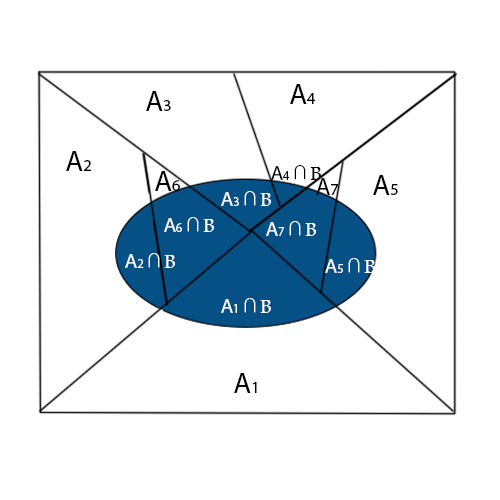
\includegraphics[scale=2]{graph/bayes_theorem.png}
\end{center}
\end{ex}
\begin{defn}
Given  $\{A_1,A_2,A_3,\cdots,A_n\}$ be a partition for the sample space $S$ and any event $B\subseteq S.$ Then, $P(A_i)$ and $P(B\mid A_i)$ for $i=1,2,3,\cdots,n$ are called \textbf{prior probabilities}
\end{defn}
\begin{thm}
Given the prior probabilities, we can calculate the \textbf{posterior probabilities}, the $P(A_j\mid B),$ $j=1,2,3,\cdots,j=1,2,3,\cdots,n$. \begin{align*}
P(A_j\mid B)&=\frac{P(A_j\cap B)}{P(B)}\\
&=\frac{P(B\mid A_j)\cdot P(A_j)}{\sum_{i=1}^nP(B\mid A_j)\cdot P(A_j)}
\end{align*}
\end{thm}
\begin{ex}
Suppose a city has two types of cabs, blue and green one. We define \begin{align*}
 P(B) &\rightarrow \text{the proportion of blue cabs in the city}\\ P(G)=1-P(B) &\rightarrow \text{the proportion of green cabs in the city}
 \end{align*}
Suppose there was a hit and run incident involving a cab in the city. With no additional information available, the probability of involved cab   is the proportion of blue cabs in the city, i.e $P(B)$\\
\hfill\\
Now, suppose we have a witness, We define \begin{align*}
 W &\rightarrow \text{event that witness says that the involved cab was a blue cab}\\
 W^c &\rightarrow \text{event that witness says that the involved cab was a green cab}
\end{align*}
Then, we have the following tree diagram\begin{center}
\begin{tikzpicture}[grow=right, sloped]
\node[bag] {}
    child {
        node[bag] {G}        
            child {
                node[end, label=right:
                    {$W^c$}] {}
                edge from parent
                node[above]  {$P(W^c\mid G)$}
            }
            child {
                node[end, label=right:
                    {$W$}] {}
                edge from parent
                node[above] {$P(W\mid G)$}
            }
            edge from parent 
            node[above] {$P(G)$}
    }
    child {
        node[bag] {B}        
        child {
                node[end, label=right:
                    {$W^c$}] {}
                edge from parent
                node[above] {$P(W^c\mid B)$}
            }
            child {
                node[end, label=right:
                    {$W$}] {}
                edge from parent
                nnode[above] {$P(W\mid B)$}
            }
        edge from parent         
            node[above] {$P(B)$}
    };
\end{tikzpicture}
\end{center}
Note that witness is correct only in the first and last case.\\
\hfill\\
Then, we want to find the probability that the involved cab was a blue cab given that the witness says it was a blue cab, i.e the posterior probability $P(B\mid W)$. Using the Bayes' Theorem, we got \begin{align*}
P(B\mid W)&=\frac{P(W\mid B)\cdot P(B)}{P(W\mid B)\cdot P(B)+P(W\mid G)\cdot P(G)}
\end{align*}
We now make prior choices for witness reliability. Let $p\in (0,1)$ be the probability that witness makes a correct observation. Then, the events corresponding to correct observations by witness $W\mid B,$ and $W^c\mid B$ has the following probabilities \begin{align*}
P(W\mid B)=P(W^c\mid G)=p
\end{align*}
Similarly, the events corresponding to incorrect observations by witness $W\mid G,$ and $W^c\mid B$ has the following probabilities \begin{align*}
P(W\mid G)=P(W^c\mid B)=1-p
\end{align*}
Let $P(B)=q\in (0,1)$. Now, we have the following update tree diagram
\begin{center}
\begin{tikzpicture}[grow=right, sloped]
\node[bag] {}
    child {
        node[bag] {G}        
            child {
                node[end, label=right:
                    {$W^c$}] {}
                edge from parent
                node[above]  {$p$}
            }
            child {
                node[end, label=right:
                    {$W$}] {}
                edge from parent
                node[above] {$1-p$}
            }
            edge from parent 
            node[above] {$1-q$}
    }
    child {
        node[bag] {B}        
        child {
                node[end, label=right:
                    {$W^c$}] {}
                edge from parent
                node[above] {$1-p$}
            }
            child {
                node[end, label=right:
                    {$W$}] {}
                edge from parent
                nnode[above] {$p$}
            }
        edge from parent         
            node[above] {$q$}
    };
\end{tikzpicture}
\end{center}
Then, \begin{align*}
P(B\mid W)&=\frac{P(W\mid B)\cdot P(B)}{P(W\mid B)\cdot P(B)+P(W\mid G)\cdot P(G)}\\
&=\frac{p\cdot q}{p\cdot q+(1-p)(1-q)}
\end{align*}
This is a beautiful equation that leads to three important cases depending on prior assumption on witness reliability, i.e the value of p.\\
\hfill\\
\textbf{Case I)} $P(B\mid W)=0$, meaning witness testimony exonerates the blue cab.
\begin{align*}
P(B\mid 0)=0&\implies \frac{pq}{pq+(1-p)(1-q)}=0\\
&\implies pq=0 \implies p=0 \text{ or }q=0
\end{align*}
$p=0$ means witness reliability is zero.\\
$q=0$ means there are no blue cabs in the city.\\
\hfill\\
\textbf{Case II)} $P(B\mid W)=1$, meaning witness testimony results in blue cab involve with complete confidence. \begin{align*}
P(B\mid W)=1&\implies \frac{pq}{pq+(1-p)(1-q)}=1\\
&\implies pq=pq+(1-p)(1-q)\implies (1-p)(1-q)=0\\
&\implies 1-p=0 \text{ or }1-q=0\\
&\implies p=1 \text{ or }q=1
\end{align*}
$p=1$ means witness is completely reliable.\\
$q=1$ means there are only blue cabs in the city.\\
\hfill\\
\textbf{Case III)} $P(B\mid W)=P(B)$, meaning witness testimony does not change our perception of the blue cab being involved.\begin{align*}
P(B\mid W)=P(B)&\implies \frac{pq}{pq+(1-p)(1-q)}=q\\
\therefore q\neq 0&\implies p=pq+(1-p)(1-q)=pq+1-p-q+pq\\
&\implies 2p-2pq=1-q \implies 2p(1-q)=(1-q)\\
\therefore (1-q)\neq 0&\implies 2p=1\implies p=\frac{1}{2}
\end{align*}
Therefore, witness testimony is independent of blue car being at faul corresponds to setting the prior witness reliability to the probability of a fair coin toss, i.e $p=\frac{1}{2}$
\end{ex}

\chapter[undecided]{undecided}
\section[Random Variables]{Random Variables}
Suppose we have an experiment with sample space $S$. We might be interested in a particular property of outcomes $\omega \in S,$ as oppsed to being interested in the outcome $\omega$ itself.
\begin{ex}
Let the experiment be tossing a two sided coin 5 times. Then \begin{align*}
|S|&=2\time 2\time 2\time 2\time 2s=2^5=32\\
S&=\{HHHHH,HHHHT,\cdots,TTTTH,TTTTT\}
\end{align*}
Then, given an $\omega\in S$, we might be interested in \begin{enumerate}[itemsep=0pt, topsep=1pt, partopsep=0pt,label=(\alph*)]
\item Number of heads in the outcome $\omega$
\item Are there at least two heads in $\omega$?
\item Is the number of heads equal to number of tails in $\omega$>
\item Are there more heads than tails in $\omega$?
\end{enumerate}
\end{ex}
\begin{ex}
Let the experiment be rolling two 6-sided dice. Then \begin{align*}
S=&\{(1,1),\cdots,(1,6),\cdots,(6,1)\cdots (6,6)\}\\
|S|=&36
\end{align*}
For any $\omega \in S$, we might be interested in \begin{enumerate}
[itemsep=0pt, topsep=1pt, partopsep=0pt,label=(\alph*)]
\item Is the sum greater than 5?
\item Is there at least one even number?
\item Is the sum divisible by 3?
\item Is the max greater than 4?
\end{enumerate}
\end{ex}
All those questions in the example above are random variable.
\begin{defn}
Let $S$ be the sample space of an experiment. A \textbf{random variable} $X$ is a function whose domain is $S$ and range is a new sample space (typically a subset of $\R$). i.e \begin{align*}
X:S&\longrightarrow \R\\
\omega &\mapsto X(\omega)
\end{align*}
The image of $X$ is the values of $X$ on the outcomes in $S$, which specify a new sample space for the original experiment in the context of a certain property, i.e $X$ extracts specific inromation about an outcome in $S$\\
Suppose $c\in X(S)$, then \begin{align*}
\{X=c\}&=\{\omega \in S:X(\omega)=c\}\\
&=\text{ All outcomes }\omega \in S\text{ which are mapped to c under X}\\
&=X^{-1}(c)
\end{align*} 
\end{defn}
\begin{thm}
Let $\X\subseteq \R$ be the set of values of $X$, then \begin{align*}
S=\bigcup_{c\in \X}\{X=c\}
\end{align*}
The subsets $\{X=c\}\subseteq S$ form a partition of $S$
\end{thm}
\begin{ex}
Suppose we toss a coin 4 times independently. Then \begin{align*}
S=\begin{Bmatrix}
HHHH & HHHT &HHTT &TTTH &TTTT\\
 &HHTH &HTHT &TTHT &\\
 &HTHH&HTTH &THTT&\\
 &THHH&THTH&HTTT&\\
 &&THHT&&\\
 &&TTHH&&
\end{Bmatrix}
\end{align*}
Let $X(\omega)=$ number of heads in the outcome $\omega$. This is a random variable $X:S\rightarrow \R$. Then, we have \begin{align*}
X(HHHT)&=3\\
X(HHHH)&=4\\
X(HTHT)=X(THTH)&=2
\end{align*}
Then let $\X=$ values of $X=\{0,1,2,3,4\}$. We can calculate $\{X=c\}$ for $c\in \X$.\begin{align*}
\{X=0\}&=\{TTTT\}\\
\{X=1\}&=\{HTTT,THTT,TTHT,TTTH\}\\
\{X=2\}&=\{HHTT,HTHT,HTTH,THTH,THHT,TTHH\}\\
\{X=3\}&=\{HHHT,HHTH,HTHH,THHH\}\\
\{X=4\}&=\{HHHH\}
\end{align*}
Then we can define the following sets with $\{X=c\}$ for $c\in \X$ \begin{align*}
 E_1&=\{X\leq 2\}=\text{ set of all outcomes with at most 2 heads}\\
 &=\{X=0\}\cup \{X=1\}\cup \{X=2\}\\
 \\
 E_2&=\{X>1\}=\text{ set of all outcomes with more than 1 heads}\\
 &=\{X=2\}\cup \{X=3\}\cup \{X=4\}\\
 &=\left(\{X=0\}\cup \{X=1\}\right)^c\\
 \\
 \{1\leq X\leq 3\}&=\text{ set of outcomes with number of heads between 1 and 3}\\
 &=\{X=1\}\cup \{X=2\}\cup \{X=3\}
\end{align*}
We can observe that in this case\begin{align*}
\bigcup_{c\in \X}\{X=c\}=S
\end{align*}
We can also define probabilities of events $\{X=c\}$ as the following \begin{align*}
P\left( \{X=c\} \right)=\sum_{\omega \in \{X=c\}}P(\omega)
\end{align*}
For example, \begin{align*}
P(X=1)&=P(\text{ Getting exactly one head in 4 independent tosses})\\
&=P(HTTT)+P(THTT)+P(TTHT)+P(TTTH)
\end{align*}
If we assume all outcomes in $S$ are equally likely, we will have \begin{align*}
P(HTTT)&=P(THTT)=P(TTHT)=P(TTTH)=\frac{1}{16}\\
\therefore P(X=1)&=4\cdot \frac{1}{16}
\end{align*}
Similarly, we can calculate \begin{align*}
P(X=0)=P(X=4)&=\frac{1}{16}\\
P(X=2)&=\frac{6}{16}\\
P(X=3)&=\frac{4}{16}
\end{align*}
These information can be organized into a table \begin{center}
\begin{tabular}{|l|l|l|l|l|l|}
\hline
$x\in \X$ & 0              & 1              & 2              & 3              & 4              \\ \hline
$P(X=x)$  & $\frac{1}{16}$ & $\frac{4}{16}$ & $\frac{6}{16}$ & $\frac{4}{16}$ & $\frac{1}{16}$ \\ \hline
\end{tabular}
\end{center}
This is also called \textbf{probability distribution table for X}.\\
Note that \begin{align*}
&P(X=0)+P(X=1)+P(X=2)+P(X=3)+P(X=4)\\
=&P\left( \bigcup_{c\in\X}\{X=c\}\right)\\
=&\frac{1}{16}+\frac{4}{16}+\frac{6}{16}+\frac{4}{16}+\frac{1}{16}\\
=&\frac{16}{16}=1\\
=&P(S)
\end{align*}
We can also define a new random variable $Y(\omega)=$ proportion of heads in the outcome. Then, \begin{align*}
Y&=\frac{\text{number of heads in an outcome}}{4}\\
&=\frac{X}{4}
\end{align*}
For example, \begin{align*}
Y(HHTT)=T(TTHH)=\frac{2}{4}
\end{align*}
\end{ex}
\begin{ex}
Let experiment be rolling a 6 sided dice 4 times. Then $|S|=6^4=16\times
 81$.\\
Define $X(\omega)=$ sum of the numbers facing up. $\X=\{4,5,\cdots,24\}$. Then \begin{align*}
 X(1,2,4,4)&=11\\
 X(1,1,1,6)&=9
 \end{align*}
Define $Y(\omega)=$ average of numbers in the sample space. Then, $\mathcal{Y}={\frac{n}{4}:n\in \N,4\leq n \leq 24}$. This is because the minimum of the average is 1 and the maximum is 6. If one of the number increases by 1, the average will increases by $\frac{1}{4}$
\end{ex}
\section[Distribution of Random Variables]{Probability Distribution of Random Variables}
\subsection[Probability Function of Random Variables]{Probability Function of Random Variables}
Given an experiment with sample space $S$. For simplicity, assume $|S|$ is finite, i.e $S=\{S_1,S_2,\cdots,S_n\}$. Let $X:S\to \R$ be a random variable, let $\X=$ values of x $=\{x_1,x_2,\cdots,x_k\}$. Then there are two sample space for the experiment
\begin{center}
\begin{tikzpicture}[grow=down, sloped]
\node[bag] {}
    child {
        node[bag] {$S$}        
            edge from parent 
    }
    child {
        node[bag] {$\X$ }        
        edge from parent         
    };
\end{tikzpicture}
\end{center}
Some simple outcomes of $S$ are $\{S_j\},j=1,2,3,\cdots,n$ and note that Events $E\subseteq S$ are described in terms of $\{S_i\}$. Some simple outcomes of $\X$ are $\{X=x_i\}=\{s\in S:X(s)=x_i\}\subseteq S$. Events $E\subset S$ are described in terms of $\{X=x_i\}$\\
Then, let $P$ be a \textbf{probability function} for S. We can use $P$ to induce a probability function $P_X$ on $\X$\\
\hfill\\
\textbf{Step 1)} \begin{align*}
P_X(\{x_i\}):=P(X=x_i)=\sum_{\omega\in \{X=x_i\}}P(\omega)
\end{align*}
Note that $\{x_i\}$ are the outcomes in $\X,$ $X=x_i$ means when the events $\omega$ in S has value of $x_i$.\\
\hfill\\
\textbf{Step 2)} Suppose $E\subseteq \X =\{x_1,x_2,x_3,\cdots,x_k\}$, then $E=\{X=x_1\}\cup \cdots \cup \{X=x_r\}$ \begin{align*}
P_X(E):=P\left(\bigcup_{i=1}^{r}\{X=x_i\} \right)=\sum_{i=1}^{r}P(X=x_i)
\end{align*}
For example, let $E=\{x_1,x_2,x_3\}$, then $E=\{X=x_1\}\cup \{X=x_2\}\cup \{X=x_3\}=\bigcup_{i=1}^3\{X=x_i\}$. Then $P_X(E)=\sum_{i=1}^3P(X=x_i)$\\
\hfill\\
\note \begin{enumerate}[itemsep=0pt, topsep=1pt, partopsep=0pt]
\item The random variable will denoted by upper case letters, $X,Y,\cdots,etc$
\item The values of the random variable will be denoted by lower cas letters, $x,y,\cdots,etc$
\item When there is no ambiguity, we will use the notation $P(X=x_i)$ instead of $P_X(X=x_i)$
\end{enumerate}
\subsection[Distribution of Random Variables]{Distribution of Random Variables}
\begin{defn}
Given an experiment with sample space $S$. Let $X$ be a random variable, $P_X$ be a probability function for X. Then, the \textbf{cumulative distribution function} of X is \begin{align*}
F_X(x)&:=P(X\leq x)\text{ }\forall x\in \X\\
F_X&:\R\longrightarrow\R\\
&x\mapsto F_X(x)=P_X(X\leq x)
\end{align*}
\end{defn}
Note that when sample space is finite \begin{align*} 
F_X(x)=P(X\leq x)=\sum_{\substack{x_i\in \X\\ x_i\leq x}}P(X=x_i)
\end{align*}
\begin{ex}
Suppose we toss a fair coin 4 times. Let $X=$ number of heads in 4  tosses. We can calculate the following:\begin{align*}
P(X=0)=\frac{1}{16}\text{, }P(X=1)=\frac{4}{16}\text{, }P(X=2)=\frac{6}{16}\text{, }P(X=3)=\frac{4}{16}\text{, }P(X=4)=\frac{1}{16}
\end{align*}
Using the above information,we can calculate $F_X(x)$ as \begin{align*}
F_X(x)=\begin{cases}
0 & \text{if }\infty<x<0\\
\frac{1}{16}& \text{if }0\leq x<1\\
\frac{5}{16}& \text{if }1\leq x<2\\
\frac{11}{16}& \text{if }2\leq x<3\\
\frac{15}{16}& \text{if }3\leq x<4\\
\frac{16}{16}=1& \text{if }4\leq x<\infty \\
\end{cases}
\end{align*}
\end{ex}
\note \begin{enumerate}[itemsep=0pt, topsep=1pt, partopsep=0pt]
\item $F_X(x)$ has jumps at $x=0,1,2,3,4$ and the jump equals $P(X=x_i)$
\item $F_X(x)$ is a non-decreasing function
\item $\lim_{x\to -\infty}F(x)=0$ and $\lim_{x\to \infty}F(x)=1$
\item $F(x)\geq 0$ $\forall x\in \R$
\end{enumerate}
\begin{thm}
A function $F(x)$ is a cumulative density function if and only if the following three conditions are satisifies: \begin{enumerate}[itemsep=0pt, topsep=1pt, partopsep=0pt, label=(\alph*)]
\item $\lim_{x\to -\infty}F(x)=0,$  $\lim_{x\to \infty}F(x)=1$
\item $F(x)$ is a non decreasing function
\item $F(x)$ is right continuous. i.e $\lim_{x\to x_o^+}F(x)=F(x_o),$ $\forall x_o\in \R$
\end{enumerate}
\end{thm}
\begin{defn}
Let X be a random variable. Then, X is \textbf{discrete} if $F_X(x)$ is a step function. Then, the probability mass function is \begin{align*}
p_X(x)=P(X=x)\text{\quad} \forall x
\end{align*}
If $x\notin \X,P(X=x)=0$
\end{defn}
\begin{defn}
Let $X$ be a random variable. Then, X is \textbf{continuous} if $F_X(x)$ is a continuous function. Then, the probability density function $f_X(x)$ satisfies \begin{align*}
\int_{-\infty}^{x}f_X(t)dt\text{\quad} \forall x
\end{align*}
\end{defn}
\begin{thm}
$f_x(x)$ is a probability density function (or probability mass function) of a random variable if and only if \begin{enumerate}
\item $f(x)\geq 0$ for all $x$
\item $\sum f_X(x)=1$ for discrete random variable or $\int_{-\infty}^{\infty}f_X(x)dx =1$ for continuous random variable
\end{enumerate}
\end{thm}
We can use cumulative density function and probability density function of a random variable $X$ to calculate $P(a\leq X\leq b)$, $P(\text{X takes values in the interval }[a,b])$
\chapter[Discrete Random Variable]{Discrete Random Variable}
Recall that $X$ is said to be a discrete random variables if and only if $F_X$ is a step function, which means $\X$ will be a discrete subset of $\R$, i.e $\X$ is a finite set, which means it is in bijection with $\{1,2,3,\cdots,N\}$ for some $N\in \N$, or countably infinite set, which means it is in bijection with $\N=\{1,2,3,4,\cdots\}$
\section[Uniform Discrete Random Variable]{Uniform Discrete Random Variable}
\begin{defn}
Fix $N\in \N$. The random variable $X$ has \textbf{uniform discrete distribution} with parameter $N$ if \begin{align*}
\X&=\{1,2,3,\cdots,N\}\\
p_X(x)&=P(X=x)=\frac{1}{N} &\text{for }x=1,2,3,\cdots,N\\
p_X(x)&=0&\text{for }x\notin \X
\end{align*}
\end{defn}
\note \begin{enumerate}
\item $\sum_{x\in \X}P_X(x)=\underbrace{\frac{1}{N}+\frac{1}{N}+\cdots+\frac{1}{N}}_{\text{N times}}=N\cdot \frac{1}{N}=1$, and $p_X(x)=\frac{1}{N}>0$ $\forall x\in \X$\\
Therefore $p_X$ is a legitimate probability mass function
\item  The distribution table for $X$ is \begin{center}
\begin{tabular}{|l|l|l|l|l|l|l|l|}
\hline
$x$      & 1             & 2             & 3             & 4             & $\cdots$ & $N-1$         & $N$a          \\ \hline
$P(X=x)$ & $\frac{1}{N}$ & $\frac{1}{N}$ & $\frac{1}{N}$ & $\frac{1}{N}$ &          & $\frac{1}{N}$ & $\frac{1}{N}$ \\ \hline
\end{tabular}
\end{center}
\item
To calculate \textbf{E(X)}\begin{align*}
E(X)&=\sum_{x\in X}x\cdot p_X(x)=\sum_{i=1}^{N}i\cdot \frac{1}{N}\\
&=\frac{1}{N}\sum_{i=1}^{N}i=\frac{1}{N}\cdot \frac{N(N+1)}{2}\\
&=\text{\colorbox{pink}{$\frac{N+1}{2}$}}
\end{align*}
\item To calculate \textbf{V(X)} we need to know that $V(X)=E(X^2)-E(X)^2$, so we want to first calculate the $E(X^2)$\begin{align*}
E(X^2)&=\sum_{x\in X}x^2\cdot p_X(x)=\sum_{i=1}^{N}i^2\cdot \frac{1}{N}\\
&=\frac{1}{N}\sum_{i=1}^{N}i^2=\frac{1}{N}\cdot \frac{N(N+1)(2N+1)}{6}\\
&=\text{\colorbox{pink}{$\frac{(N+1)(2N+1)}{6}$}}
\end{align*}
Therefore, $V(X)$ is \begin{align*}
V(X)&=E(X^2)-E(X)^2=\frac{(N+1)(2N+1)}{6}-\left(\frac{N+1}{2} \right)^2\\
&=\text{\colorbox{pink}{$\frac{(N+1)(N-1)}{12}$}}=\left(\frac{N^2-1}{12} \right)
\end{align*}
\item At $\{a_1,a_2,\cdots,a_n\}\subseteq \R$, we define \begin{align*}
h:\X &\longrightarrow \{a_1,a_2,\cdots,a_N\}\\
i&\mapsto a_i
\end{align*}
Then if $X$ has uniform distribution, $E(h(x))=\frac{a_1+a_2+\cdots+a_N}{N}$, and $V(h(x))=$ variance of the numbers $\{a_1,a_2,\cdots,a_N\}=\frac{1}{N}\sum_{i=1}^{N}(a_i-M)^2$
\end{enumerate}
\section[Binomial Distribution]{Binomial Distribution}
Fix $N,M,n\in \N$. Suppose a bag has $N$ balls that are identical except for color and $M$ of them are read. Let the experiment be choosing n balls from the bag and define a random variable $X=$ number of red balls in the sample of n balls.\\
If we want to calculate $p_X(x)=P(X=x),$ we first need to know if there is replacement or not. If it is sampling with replacement, then it is a binomial distribution with parameters: $n,p=\frac{M}{N}$. If without replacement, it is a hypergeometric distribution, which we will discuss later. \begin{defn}
X is said to have \textbf{Binomial Distribution} with parameters: $n,p$ if \begin{align*}
\X&=\{0,1,2,\cdots,n\}\\
p_X(x)&=\binom nx \cdot p^x\cdot (1-p)^{n-x}
\end{align*}
\note \begin{enumerate}
\item \begin{align*}
\sum_{x\in \X}p_X(x)&=\sum_{x=0}^{n}\binom nx p^x\cdot (1-p)^{n-x}\\
&=(p+(1-p))^n=1^n=1
\end{align*}
Therefore, $p_X$ is a probability mass function.
\item To calculate \textbf{E(X)}\begin{align*}
E(X)=\text{\colorbox{pink}{$n\cdot p$}}
\end{align*}
\item To calculate \textbf{V(X)}\begin{align*}
V(X)=\text{\colorbox{pink}{$n\cdot p \cdot (1-p)$}}
\end{align*}
\end{enumerate}
\end{defn}
\section[Hypergeometric Distribution]{Hypergeometric Distribution}
Reacall that if the choosing balls experiment mentioned in the binomial distribution is sampling without replacement, then it is a hypergeometric distribution with parameters: $N,M,n$.
\begin{defn}
X is said to have \textbf{hypergeometric distribution} with parameters:  $N,M,n$ if \begin{align*}
\X&=\{0,1,2,3,\cdots,n\}\\
p_X(x)=P(X=x)&=\frac{\binom Mx \cdot \binom{N-M}{n-x}}{\binom Nn}
\end{align*} 
Note that $P(X=x)$ is the probability of getting exactly $x$ successes in a sample of size $n$ without replacement from a population of size $N$ with $M$ successes.
\end{defn}
\note \begin{enumerate}
\item $x$ must satisfy the following condition \begin{center}
$max(0,n-N+M)\leq x\leq min(n,M)$
\end{center}
where $n$ is the sample size, $N$ is the population, $M$ is the number of successes. 
\item To calculate $E(X)$\begin{align*}
E(X)=n\cdot \frac{M}{N}
\end{align*}
\item To calculate $V(X)$\begin{align*}
V(X)=\left(\frac{N-n}{N-1} \right)\cdot n\cdot \left(\frac{M}{N}\right)\cdot \left(1-\frac{M}{N} \right)
\end{align*}
\item If $N$ is large enough, then $\frac{N}{M}\to p$, so we can use the Hypergeometric distribution$(N,M,n)$ to approximate Binomial $(N,p=\frac{M}{N})$. Then if we set $p=\frac{M}{N}$ \begin{align*}
E(X)&=n\cdot p\\
V(X)&=\frac{N-n}{N-1}\cdot n\cdot p \cdot(1-p)=n\cdot p \cdot(1-p) \text{ since }n\to \infty, \frac{N-n}{N-1}\approx 1
\end{align*}
\end{enumerate}
\section[Bernoulli Distribution]{Bernoulli Distribution}
If an experiment has exactly two outcomes, and the probability of success is $p$ and failure is $(1-p)$, then we said $X$ is a bernolli random variable.\begin{defn}
X is a \textbf{Bernolli} random variable with parameter $p$ if \begin{align*}
\X&=\{0,1\}\\
p_X(\X)&=\begin{cases}
p &\text{if }x=1\\
(1-p) &\text{if }x=0
\end{cases}
\end{align*}
Then we have \colorbox{pink}{$E(X)=p$} and \colorbox{pink}{$V(X)=p\cdot (1-p)$}
\end{defn}
\section[Poisson Distribution]{Poisson Distribution}
Now, we want to study discrete random variables which have $\X$ to be infinte. \begin{defn}
X is said to have \textbf{Poisson Distribution} with parameter $\lambda >0$ if \begin{align*}
\X&=\{0,1,2,3,\cdots\}\\
p_X(x)&=\frac{e^{-\lambda}\cdot \lambda^x}{x!}\text{ for }x\in \X
\end{align*}
\end{defn} 
\note \begin{enumerate}
\item \begin{align*}
e^{\lambda}&=1+\lambda+\frac{\lambda^2}{2!}+\cdots\\
&=\sum_{x=0}^{\infty}\frac{\lambda^x}{x!}\\
\implies 1&=e^{-\lambda}\cdot \sum_{x=0}^{\infty}\frac{\lambda^x}{x!}=\sum_{x=0}^{\infty}e^{-\lambda}\cdot\frac{\lambda^x}{x!}=\sum_{x=0}^{\infty}p_X(x)
\end{align*}
Also, $p_X(x)=\frac{e^{-\lambda}\cdot \lambda^x}{x!}\geq 0$ for all $x\in \X$. Therefore, $p_X$ is a legitimate probability mass function. 
\item The mean and variance are\begin{align*}
&\text{\colorbox{pink}{$E(X)=M_x=\lambda$}}\\
&\text{\colorbox{pink}{$V(x)=\sigma_X^2=\lambda$}}\\
&\text{\colorbox{pink}{$\sigma_X=\sqrt{\lambda}$}}
\end{align*}
\item The Poisson distribution is often used to model phenomena where we are waiting for events to happen.
\end{enumerate}
\section[Negative Binomial Distribution]{Negative Binomial Distribution}
\begin{defn}
X is said to have \textbf{Negative Binomial Distribution} with parameters $r,p$ if \begin{align*}
\X&=\{0,1,2,3,\cdots\}\\
p_X(x)&=\binom{x+r-1}{r-1}p^r\cdot (1-p)^x\text{ for }x\in \X
\end{align*}
\end{defn}
\note \begin{enumerate}
\item The experiment for Negative Binomial Distribution is performing Bernoulli trials with P(success) = p repeatedly until we get exactly r successes.\\
Let X = number of failure that precede the $r^{th}$ successes, then \begin{align*}
P(X=x)&=P(\text{Exactly $x$ failures before $r^{th}$ successes})
\end{align*}
And the total ways we can have exactly $x$ failures before $r^{th}$ successes is choosing $x$ spots in $x+r-1$ possible places, since the last spot has to be a successes. Then, there are  \begin{align*}
\binom{x+r-1}{x}&=\binom{x+r-1}{r-1} \text{ ways}
\end{align*}
Therefore, \begin{align*}
p_X(x)&=\binom{x+r-1}{r-1}p^r\cdot (1-p)^x
\end{align*}
\item The mean and variance are \begin{align*}
&\text{\colorbox{pink}{$E(X)=\mu_x=\frac{r(1-p)}{p}$}}\\
&\text{\colorbox{pink}{$V(x)=\sigma_X^2=\frac{r(1-p)}{p^2}$}}
\end{align*}
\item We called it negative binomial distribution because \begin{align*}
\binom{x+r-1}{x}=(-1)^x \binom{-r}{x}
\end{align*}
Therefore, \begin{align*}
p_X(x)=(-1)^x\binom{-r}{x}p^r(1-p)^x
\end{align*}
Note that $\binom{-r}{x}p^r(1-p)^x$ is very similar to the probability mass function of Binomial Distribution
\end{enumerate}
\section[Geometric Distribution]{Geometric Distribution}
\begin{defn}
We say X has \textbf{Geometric Distribution} with parameter p if \begin{align*}
\X&=\{0,1,2,3,\cdots\}\\
p_X(x)&=p(1-p)^{x-1}\text{ for }x\in \X
\end{align*}
\end{defn}
\note \begin{enumerate}
\item The Geometric distribution is a special case of Negative Binomial distribution when $r=1$. It is the simplest of the waiting time distribution where $X$ can be interpreted as the trial at which first successes occurs, which is "waiting for a success."\\
\item The mean and variances are \begin{align*}
&\text{\colorbox{pink}{$E(X)=\mu_x=\frac{1}{p}$}}\\
&\text{\colorbox{pink}{$V(x)=\sigma_X^2=\frac{(1-p)}{p^2}$}}
\end{align*}
\item Sometimes it is used to moedl lifetime or time until failure of components
\end{enumerate}
\section[Relationships Between Discrete Distributions]{Relationships Between Discrete Distributions}
\subsection[Binomial and Hypergeometric]{Binomial and Hypergeometric}
Let $N,M,n\in \N$ be given and set $p=\frac{M}{N}$. Then, \begin{enumerate}[itemsep=0pt, topsep=1pt, partopsep=0pt,label=(\alph*)]
\item bin$(x;n,p)$ is the probability mas function for binomial distribution with parameters: \begin{align*}
n&=\text{ sample size}\\
p&=\text{ probability of success}
\end{align*}
\item hyper$(x;N,M,n)$ is the probability mass function for hypergeometric distribution with parameters\begin{align*}
n&=\text{ sample size}\\
M&=\text{number of successes}\\
N&=\text{population size}
\end{align*}
Then, if $N,M\to \infty$, and $\frac{M}{N}\to p$, then hyper$(x;N,M,n)\to$bin$(x;n,p)$, i.e if sample size N is small compared to population size $N$, we can assume that samples are approximately independent.
\end{enumerate}
\subsection[Binomial and Poisson]{Binomial and Poisson}
Suppose \begin{enumerate}[itemsep=0pt, topsep=1pt, partopsep=0pt,label=(\alph*)]
\item bin$(x;n,p)$ is the probability mas function for binomial Distribution with parameters: \begin{align*}
n&=\text{ sample size}\\
p&=\text{ probability of success}
\end{align*}
\item pois$(x;\lambda)$ is the probability mass function for Poisson Distribution with parameters $\lambda>-$
\end{enumerate}
Then, if $n\to \infty$ and $p\to 0$ such that $n\cdot p\to \lambda$, then then bin$(x;N,M,n)\to$ pois$(x;n,p)$, i.e If $n$ is large and $p$ is small, bin$(x;N,M,n)\approx$ pois$(x;n,p)$, or the Poisson Distribution is approximately Binomial fore rare events. 
\chapter[Continuous Random Variable]{Continuous Random Variable}
\section[Introduction]{Introduction}
Recall that $X$ is a continuous random variable if and only if the cumulative density function $F_x$ is a continuous function.\\ 
Let $f_X(x)$ be the probability density function of $X$ which satisfies the following \begin{align*}
F_X(x)=\int_{-\infty}^{x}f_x(t)dt
\end{align*}
\note \begin{enumerate}
\item $f_X(x)$ must satisfy:\begin{enumerate}[itemsep=0pt, topsep=1pt, partopsep=0pt,label=(\alph*)]
\item $f_X(x)\geq 0$ for all $x\in (-\infty,\infty)$
\item $\int_{-\infty}^{\infty}f_X(x)dx=1$
\end{enumerate}
\item The expected value of $X$ is \begin{align*}
&\text{\colorbox{pink}{$E(X)=\mu_x=\int_{-\infty}^{\infty}xf_X(x)dx$}}\\
\end{align*}
\item The variance of $X$ is\begin{align*}
&\text{\colorbox{pink}{$V(X)=\sigma_X^2=\int_{-\infty}^{\infty}(x-\mu_x)^2f_X(x)dx$}}\\
\end{align*}
\item The standard deviation of $X$ is \begin{align*}
&\text{\colorbox{pink}{$\sigma_X=\sqrt{\sigma_X^2}$}}\\
\end{align*}
\item Variance can be also written as following\begin{align*}
V(X)=E(X^2)-(E(X))^2
\end{align*}
\item There is one important identities associates with the expected value function \begin{align*}
\text{\colorbox{yellow}{$E(h(X))=\int_{-\infty}^{\infty}h(x)f_X(x)dx$}}\\
\end{align*}
for example, \begin{align*}
E(aX+b)=aE(X)+b\text{, }V(aX+b)=a^2V(X)
\end{align*}
\end{enumerate} 
To calculate the probabilities for the events we want, we need to use the cumulative density function that is defined as the following \begin{align*}
F_X(x):=P(X\leq x)=\int_{-\infty}^{x}f_X(t)dt
\end{align*}
i.e $F_X(x)$ is the area under graph of $f_X$ upto x. \\
\hfill\\
\note \begin{enumerate}
\item \begin{align*}
P(a\leq X\leq b)&=\int_{a}^{b}f_X(x)dx \text{ }a\leq b\\
&=\int_{-\infty}^{b}f_X(x)dx-\int_{-\infty}^{a}f_X(x)dx\\
&=F_X(b)-F_X(a)
\end{align*}
\item The probability that a continious random variable take a particular value is zero\begin{align*}
P(X=c)=P(c\leq x \leq c)=F_X(c)-F_X(c)=0
\end{align*}
\item \begin{align*}
P(X>c)=&1-P(x\leq c)=1-F_X(c)\\
P(X\geq c)=&P(X>c)+P(X=c)=P(X>c)
\end{align*}
\end{enumerate}
And we can use the cumulative density function $F_X$ to calculate $f_X(x).$ If the derivative $F_X'(x)$ exist at $x$, then \begin{align*}
F_X'(x)=f_X(x)
\end{align*}
Let $p\in (0,1).$ Then the "$(100\cdot p)th$" Percentile for the distribution of X is $\eta(p)$ and satisfies \begin{align*}
p=F_X(\eta (p))=\int_{-\infty}^{\eta (p)}f_X(x)dx
\end{align*}
Let $\alpha\in (0,1)$. Then the the $\alpha th$ critical value for the distribution of $X$ is $\X_{\alpha}$ and satisfies\begin{align*}
\alpha = P(X>X_{\alpha})=1-F_X(x\alpha)
\end{align*}
Note that $(100p)th$ percentile is same as $(1-p)6h$ critical value.
\section[Uniform Continuous Distribution]{Uniform Continuous Distribution}
Let $[A,B]\subseteq \R$ be a closed interval where $A<B$. Then we can define the probability density function as the following \begin{align*}
f(x)&=\begin{cases}
\frac{1}{B-A} &x\in [A,B]\\
0 &\text{otherwise}
\end{cases}
\end{align*}
Then, the cumulative density function of the uniform continuous distribution  is \begin{align*}
F(x)=\begin{cases}
0 &\text{if }x<A\\
\frac{x-A}{B-a} &<\text{if }x\in [A,B]\\
1 &\text{if } x\geq B
\end{cases}
\end{align*}
Then, the expected value is \begin{align*}
E(X)&=\int_{-\infty}^{\infty}x\cdot f(x)dx=\int_{A}^{B}\frac{x}{B_A}dx\\
&=\text{\colorbox{pink}{$\frac{B+A}{2}$}}\\
\end{align*}
The variance is \begin{align*}
V(X)&=\int_{-\infty}^{\infty}(x-\mu_x)^2f_X(x)dx=\int_{A}^{B}\frac{\left(x-\frac{B+A}{2}\right)^2}{B_A}dx\\
&=\text{\colorbox{pink}{$\frac{(B+A)^2}{12}$}}\\
\end{align*}
If $a,b\in [A,B]$ and $a<b$, then \begin{align*}
P(a\leq X\leq b)=\int_{a}^{b}\frac{x}{B-a}=\frac{b-a}{B-A}
\end{align*}
\section[Normal Distribution]{Normal Distribution}
\begin{defn}
We define \textbf{Normal Distribution} using the following two parameters \begin{align*}
M &\to \text{ mean}\\
\sigma^2 &\to \text{ variance} 
\end{align*}
denoted as $N(M,\sigma^2)$
\end{defn}
\note $\sigma = \sqrt{\sigma^2}$ is the standard deviation.\begin{defn}
Suppose $X$ is normally distributed, i.e $X\sim N(M,\sigma^2)$. Then, the probability density function of X is defined as \begin{align*}
f(x)&=\frac{1}{\sqrt{2\pi}\sigma}\cdot e^{\frac{-(x-M)^2}{2\sigma^2}}, \text{ }x\in (-\infty, \infty)
\end{align*}
And the cumulative density function is \begin{align*}
F(x)=P(X\leq x)=\int_{-\infty}^{x}f(t)dt=\frac{1}{\sqrt{2\pi}\sigma}\int_{-\infty}^{x} e^{\frac{-(t-M)^2}{2\sigma^2}}dt
\end{align*}
Therefore, \begin{align*}
P(a\leq X \leq b)=\frac{1}{\sqrt{2\pi}\sigma}\int_{a}^{b} e^{\frac{-(t-M)^2}{2\sigma^2}}dt
\end{align*}
\end{defn}
\note \begin{enumerate}
\item If $x\sim N(M,\sigma^2),$ then \begin{align*}
E(X)&=\text{\colorbox{pink}{$M$}}\\
V(X)&=\text{\colorbox{pink}{$\sigma^2$}}
\end{align*}
\item When $M=0,\sigma^2=1$, it is a \textbf{Standard Normal Distribution} $Z\sim N(0,1)$, and the standard normal distribution probability density function is \begin{align*}
f(z)&=\frac{1}{\sqrt{2\pi}}\cdot e^{\frac{-z^2}{2}}, \text{ }x\in (-\infty, \infty)
\end{align*}
and the cumulative density function of $Z$ is denoted as $\Phi(z)$, \begin{align*}
P(Z\leq z)=\Phi(z)=\frac{1}{\sqrt{2\pi}}\int_{-\infty}^{z} e^{\frac{-t^2}{2}}dt
\end{align*}
To be specific about parameters, we denote probability density function of $X\sim N(M,\sigma^2)$ as \begin{align*}
f(x;M,\sigma^2)=\frac{1}{\sqrt{2\pi}\sigma}\cdot e^{\frac{-(x-M)^2}{2\sigma^2}}, \text{ }x\in (-\infty, \infty)
\end{align*}
\item If $X\sim N(M,\sigma^2)$ and $Z\sim N(0,1)$, then \begin{align*}
P(X\leq x)&=\frac{1}{\sqrt{2\pi}\sigma}\int_{-\infty}^{x} e^{\frac{-(t-M)^2}{2\sigma^2}}dt\\
&=\frac{1}{\sqrt{2\pi}}\int_{-\infty}^{\frac{x-M}{\sigma}} e^{\frac{-s^2}{2}}ds &\text{Change of vaiable with }s=\frac{t-M}{\sigma}\\
&=P(z\leq \frac{x-M}{\sigma})
\end{align*}
Therefore, if $X\sim N(M,\sigma^2)$, then $\frac{X-M}{\sigma}$ has the standard normal distribution.
\item If $X\sim N(M,\sigma^2)$, then $Z=\frac{X-M}{\sigma}\sim N(0,1)$. Then \begin{align*}
P(a\leq X\leq b)&=P\left(\frac{a-M}{\sigma}\leq z\leq \frac{b-M}{\sigma} \right)\\
&=\Phi \left(\frac{b-M}{\sigma} \right)-\Phi\left(\frac{a-M}{\sigma} \right)
\end{align*}
Therefore, we can use the standard normal cumulative density function to calculate probability for the random variable $X\sim N(M,\sigma^2)$, i.e \begin{align*}
\text{\colorbox{yellow}{$X\sim N(M,\sigma^2)$}}&\longrightarrow \text{\colorbox{yellow}{$Z\sim N(0,1)$}}\\
x&\mapsto Z=\frac{x-M}{\sigma}\text{\qquad It is also Z-score of }x \\
z&\mapsto x=Z\cdot \sigma+M 
\end{align*}
\end{enumerate}
\subsection[Percentile and Critical Values]{Percentile and Critical Values}
\begin{defn}
Suppose $Z\sim N(0,1)$, the standard normal distribution. Then, for $\alpha \in (0,1),z_{\alpha}$ is the $\alpha th$ \textbf{critical value} that satisfies the following \begin{align*}
P(Z\geq z_{\alpha}) &=\alpha\\
\text{i.e \qquad} \int_{z_{\alpha}}^{\infty}f(z;0,1)dz&=\alpha\\
\text{i.e \quad} 1-P(Z\leq z_{\alpha})=\alpha&\implies 1-\Phi(z_{\alpha})=\alpha
\end{align*}
\end{defn}
\begin{defn}
Let $p\in (0,1)$. Then $(100p)th$ \textbf{percentile}, $\eta (p)$ satisfies \begin{align*}
P(Z\leq \eta (p))&=p\\
\text{i.e \quad}\Phi(\eta(p))&=p
\end{align*} 
\end{defn}
Suppose $X\sim N(M,\sigma^2)$ and $\alpha \in (0,1)$, then \begin{align*}
\alpha^{th}\text{ critical value for }X&:= x_{\alpha}=\sigma z_{\alpha}+M 
\end{align*}
where $z_{\alpha}$ is the $\alpha^{th}$ critical value for $Z\in N(0,1)$
\subsection[Approximating Bin(n,p) using Normal Distribution]{Approximating Bin(n,p) using Normal Distribution}
Let $X\sim Bin(n,p)$, i.e $\mu_x=np$ and $\sigma_x^2=np(1-p)$. Then if the $Bin(n,p)$ is not too skewed, then \begin{align*}
P(X\leq x)\approx \Phi \left(\frac{x+0.5-Mx}{\sigma_x} \right)
\end{align*}
The right hand side does not involve terms of the form $\binom nk$, which can be difficult to compute.
\section[Gamma Distribution]{Gamma Distribution}
Gama distribution is useful when modeling component lifetimes and waiting times. \begin{defn}
\textbf{Gamma function} is defined as \begin{align*}
\Gamma(\alpha)=\int_{0}^{\infty}t^{\alpha-1}\cdot e^{-t}dt,\text{ for }\alpha >0
\end{align*}
\end{defn}
\begin{thm}
\textbf{Properties of Gamma Function}\begin{enumerate}
\item $\Gamma(\alpha+1)=\alpha \Gamma(\alpha)$ for $\alpha >0$. Since $\Gamma(1)=1$, we have $\Gamma(n)=(n-1)!$ for $n\in \N$ using induction
\item $\Gamma(\frac{1}{2})=\sqrt{\pi}$
\end{enumerate}
\end{thm}
\begin{defn}
We say $X$ has the \textbf{Gamma Distribution} with shape parameter $\alpha$ and scale parameter $\beta$ if the probability density function of $X$ is \begin{align*}
f(x;\alpha,\beta)=\begin{cases}
\frac{1}{\beta^{\alpha}\Gamma(\alpha)}x^{\alpha-1}\cdot e^{\frac{-x}{\beta}} & x> 0\\
0 & x\leq 0
\end{cases}
\end{align*}
\end{defn}
Since $f(x;\alpha,\beta)\geq 0$ $\forall x\in \R$ and we can check $\int_{-\infty}^{\infty}f(x;\alpha,\beta)dx=1$ by doing a change of variable $y=\frac{x}{\beta}$, therefore $f$ satisfies the property of probability density function.\\
\hfill\\
\note \begin{enumerate}
\item When $\beta=1$, we call it a \textbf{standard gamma distribution} with shape parameters $\alpha$, with probability density function \begin{align*}
f(x;\alpha)&=\begin{cases}
\frac{x^{\alpha-1}e^{-x}}{\Gamma(\alpha)}& x> 0\\
0 & x\leq 0
\end{cases}
\end{align*}If $T$ has standard Gamma distribution with shape parameters: $\alpha$, then $X=\beta T$ has Gamma distribution with shape $\alpha$, and scale $\beta$
\item If $X\sim Gamma(\alpha,\beta),$ then \begin{enumerate}
\item \colorbox{pink}{$E(X)=\mu_x=\alpha \beta$}
\item \colorbox{pink}{$V(X)=\sigma_X^2=\alpha \beta^2$}
\item \colorbox{pink}{$\sigma=\sqrt{\alpha} \beta$}
\end{enumerate}
\item The cumulative density function of $X\sim Gamma(\alpha,\beta)$ is the following \begin{align*}
F_X(x;\alpha,\beta)&=\begin{cases}
\int_{0}^{x}f(t;\alpha,\beta)dt &\text{if }x>0\\
0 &\text{otherwise}
\end{cases}
\end{align*}
Then $P(X\leq x)=F_X(x;\alpha,\beta)=F\left(\frac{x}{\beta};\alpha \right)$, the cumulative density function of standard Gamma with parameters $\alpha$, i.e \begin{align*}
F_X(x;\alpha)&=\begin{cases}
\int_{0}^x\frac{t^{\alpha-1}e^{-t}}{\Gamma(\alpha)}& \text{if }x\geq 0\\
0 & \text{otherwise}
\end{cases}
\end{align*}
\end{enumerate}
\subsection[Special Cases of Gamma Distribution]{Special Cases of Gamma Distribution}
\begin{defn}
When $X$ has a Gamma Distribution with $\alpha=1,\Gamma-\frac{1}{\lambda}$ for some $\lambda>0$. Then, we say $X$ has a \textbf{Exponential Distribution} with parameter $\lambda$. The probability density function of $X$ is the \begin{align*}
f(x;\lambda)&=\begin{cases}
\lambda \cdot e^{-\lambda x}&\text{if }x\geq 0\\
0&\text{otherwise}
\end{cases}
\end{align*}
And the cumulative density function of $X$ \begin{align*}
F_X(x;\lambda)&=\begin{cases}
1-e^{-\lambda x}&\text{if }x\geq 0\\
0&\text{otherwise}
\end{cases}
\end{align*}
\end{defn}
\note \begin{enumerate}
\item If $X$ has exponential distribution with parameters $\lambda>0$, hen \begin{enumerate}
\item \colorbox{pink}{$E(X)=\mu_x=\frac{1}{\lambda}$}
\item \colorbox{pink}{$V(X)=\sigma_X^2=\frac{1}{\lambda^2}$}
\item \colorbox{pink}{$\sigma=\frac{1}{\lambda}$}
\end{enumerate}
\item If we have a Poisson process with rate $\alpha$, then the exponential distribution with $\lambda=\alpha$ models the distribution of elapsed time between the occurrence of two successive events.
\item If $X\sim Exp(\lambda)$, then \begin{align*}
P(X\geq t+t_0\mid X\geq t_0)&=\frac{[\{X\geq t+t_0\}\cap\{X\geq t_0\} ]}{P(X\geq t_0)}\\
&=\frac{P(X\geq t+t_0)}{P(X\geq t_0)}=\frac{1-F(t+t_0;\lambda)}{1-F(t_0;\lambda)}\\
&=e^{-\lambda t}=P(X\geq t)
\end{align*}
This means that if $X$ was modeling lifetime of a component, the distribution of additional lifetime is exactly the same as the original distribution of lifetime, i.e the exponential distribution has \textbf{meaningless property}  
\end{enumerate}
\begin{defn}
$X$ is said to have \textbf{chi-squared} distribution with parameter $\upsilon$ (degress of freedom) if $X\sim Gamma(\alpha,\beta)$ with $\alpha=\frac{\upsilon}{2},\beta=2$. The probability density function of $X$ is defined as the following \begin{align*}
f(x;\upsilon)&=\begin{cases}
\frac{1}{2^{\frac{\upsilon}{2}}\cdot \Gamma\left(\frac{\upsilon}{2}\right)}\cdot x^{\frac{\upsilon}{2}-1}\cdot e^{\frac{-x}{2}}&\text{if }x\geq 0\\
0&\text{otherwise}
\end{cases}
\end{align*}
\end{defn}
\note \begin{enumerate}
\item If $X$ is a chi-squared distribution with parameters $\upsilon$, then\begin{enumerate}
\item \colorbox{pink}{$E(X)=\mu_x=\alpha \cdot \beta=\upsilon$}
\item \colorbox{pink}{$V(X)=\sigma_X^2=\alpha \beta^2=2\upsilon$}
\item \colorbox{pink}{$\sigma=\sqrt{2\upsilon}$}
\end{enumerate}
\item Chi-square distribution plays important role in statistical inference.
\item If $X\sim N(M,\sigma^2)$, then $\left(\frac{X-M}{\sigma} \right)^2$ has chi-square distribution with $\upsilon=1$
\end{enumerate}
\section[Lognormal Distribution]{Lognormal Distribution}
\begin{defn}
We say $X$ has a \textbf{Lognormal Distribution} if $\ln(X)$ has normal distribution with parameters $M$ and $\sigma^2$. i.e \begin{align*}
\ln(X)\sim N(M,\sigma^2)
\end{align*}
If $X$ has lognormal distribution, then the probability density function is \begin{align*}
f(x;M,\sigma)=\begin{cases}
\frac{1}{\sqrt{2\pi}\sigma x}\cdot e^{\frac{-(\ln(x)-M)^2}{2\sigma^2}} & \text{if }x\geq 0\\
0 & \text{otherwise}
\end{cases}
\end{align*}
\end{defn}
\note \begin{enumerate}
\item If $\sim N(M,\sigma^2)$ then\begin{enumerate}
\item \colorbox{yellow}{$E(\ln(X))=M$}
\item \colorbox{yellow}{$V(\ln(X))=\sigma^2$}
\end{enumerate}
\item If $X$ has lognormal distribution, and $\ln(x)\sim N(M,\sigma^2)$, then \begin{enumerate}
\item \colorbox{pink}{$E(X)=\mu_x=e^{M+\frac{\sigma^2}{2}}$}
\item \colorbox{pink}{$V(X)=\sigma_X^2=e^{(2M+\sigma^2)}\cdot (e^{\sigma^2}-1)$}
\end{enumerate}
\item We can use standard normal table to calculate the probabilities \begin{align*}
F_X(x;M,\sigma)&=P(X\leq x)=P(\ln(x)\leq \ln(x))\\
&=P(Z\leq \frac{\ln(x)-M}{\sigma}) \text{\qquad }\because \ln(x)\sim N(M,\sigma^2)\\
&=\Phi\left(\frac{\ln(x)-M}{\sigma} \right)\text{\qquad for }x>0 
\end{align*}
\end{enumerate}
\section[Beta Distribution]{Beta Distribution}
Beta distribution takes values in a finite interval, which is good to model proportions that naturally lie in $(0,1)$\begin{defn}
$X$ is said to have \textbf{Beta Disribution} with parameters:$\alpha,\beta>0$ if the probability density function is \begin{align*}
f(x;\alpha,\beta)&=\frac{\Gamma(\alpha+\beta)}{\Gamma(\alpha)\Gamma(\beta)}\cdot x^{\alpha -1}(1-x)^{\beta -1} \text{\qquad}x\in (0,1)
\end{align*}
\end{defn}
\note \begin{enumerate}
\item We called Beta distribution be cause the Beta function is \begin{align*}
B(\alpha,\beta)&=\frac{\Gamma(\alpha)\cdot \Gamma(B)}{\Gamma(\alpha+\beta)} \text{\qquad for }\alpha,\beta>0
\end{align*}
So that \begin{align*}
f(x;\alpha,\beta)&=\frac{1}{B(\alpha,\beta)}\cdot x^{\alpha -1}(1-x)^{\beta -1} \text{\qquad}x\in (0,1)
\end{align*}
\item If $X\sim Beta(\alpha,\beta)$, then \begin{enumerate}
\item \colorbox{pink}{$E(X)=\mu_x=\frac{\alpha}{\alpha+\beta}$}
\item \colorbox{pink}{$V(X)=\sigma_X^2=\frac{\alpha \beta}{(\alpha+\beta)^2(\alpha+\beta+1)}$}
\end{enumerate}
Note that both $\mu_x$ and $\sigma_X^2$ are in $(0,1)$
\item Depending on values of $\alpha,\beta$, the probability density function $f(x;\alpha,\beta)$ has different shapes.  \begin{enumerate}
\item If $\alpha>1,\beta =1$, then it is strictly increasing
\item If $\alpha=1,\beta >1$, then it is strictly decreasing
\item If $\alpha<1,\beta <1$, then it is U-shaped
\item If $\alpha=\beta$, then it is symmetric about $\frac{1}{2}$ with $\mu_x=\frac{1}{2}$ and $\sigma_X^2=\frac{1}{4(2\alpha+1)}$
\item If $\alpha=\beta=1$, then it is a uniform distribution on $(0,1)$
\end{enumerate}
\end{enumerate}
\section[Cauchy Distribution]{Cauchy Distribution}
\begin{defn}
$X$ is said to have \textbf{Cauchy Distribution} with parameter $\theta$ if the probability density function of $X$ is \begin{align*}
f(x;\theta)=\frac{1}{\pi}\cdot \frac{1}{1+(x-\theta)^2}&x\in (-\infty,\infty)\\
&\theta\in (-\infty,\infty)
\end{align*}
\end{defn}
\note \begin{enumerate}
\item $E(X)$ and $V(X)$ do not exists if $X$ has Cauchy distribution since \begin{align*}
E(X)=\int_{-\infty}^{\infty}xf(x)dx&=\int_{-\infty}^{\infty}\frac{1}{\pi}\cdot \frac{x}{1+(x-\theta)^2}dx\\
&=0\text{ since } \frac{x}{1+(x-\theta)^2}\text{ is an odd function}
\end{align*}
This is not the case.
\item The graph of $f(x;\theta)$ is bell shaped like the Normal density but has heavier tails than Normal density.
\end{enumerate}
\chapter[Joint Distribution]{Joint Distribution}
Many experiment or applications require that we use more than one characteristic or variable related to the experimental unit. For example:\begin{enumerate}
\item Studying Body Mass Index (BMI) need the height and the weight
\item Predicating house prices need many factors: location, house area, number of bedroom and bathrooms, etc.
\item Predicting the price of a stock depends on many performance metrics - perhaps how Elon tweets
\end{enumerate}
In all these cases, we nee to calculate the probability of two or more events simultaneously, therefore, we want the \textbf{Joint Distribution} of variable of interest
\section[Two Discrete Random Variable]{Two Discrete Random Variable}
\begin{defn}
Suppose $X,Y$ are two discrete random variables. Then $\mathcal{X}:=$ values of $X$ and $\mathcal{Y}:=$ values of $Y$. Then, the cartesian product of $\mathcal{X},\mathcal{Y}$\begin{align*}
\mathcal{X}\times \mathcal{Y}&=\{(x,y):x\in \mathcal{X},y\in \mathcal{Y}\}
\end{align*}
is the \textbf{Joint Sample Space}.\\
The \textbf{Joint Probability Mass Function}, i.e Joint pmf of $X$ and $Y$ is \begin{align*}
P(x,y):=P(X=x \text{ and }Y=y)
\end{align*}
Which is $P($ X takes value $x$ and Y takes value $y$ $)$
\end{defn}
\note \begin{enumerate}
\item $p(x,y)$ satisfies \begin{enumerate}
\item $p(x,y)\geq 0$ $\forall(x,y)\in \mathcal{X}\times \mathcal{Y}$
\item $\sum_{(x,y)\in \mathcal{X}\times \mathcal{Y}}=1$
\end{enumerate}
\item If $A\subseteq \mathcal{X}\times \mathcal{Y}$, i.e A is a set of events in the joint distribution, then \begin{align*}
P(A)=\sum_{(x,y)\in A}p(x,y)
\end{align*}
\end{enumerate}
\begin{defn}
Given a joint sample space of $X,Y$, we define the \textbf{Marginal Probability Mass Function of }$X$ as \begin{align*}
p_X(x)&:=\sum_{y\in \mathcal{Y}}p(x,y) \text{ for fixed }x\in \mathcal{X}
\end{align*}
\textbf{Marginal Probability Mass Function of }$Y$ as \begin{align*}
p_Y(y)&:=\sum_{x\in \mathcal{X}}p(x,y) \text{ for fixed }y\in \mathcal{Y}
\end{align*}
\end{defn}
\begin{defn}
Given a joint sample space of $X,Y$, we define the \textbf{conditional distribution function} of $X$ given that $Y=y$ as \begin{align*}
p_{X\mid Y}&:=P(X=x \text{ given that }Y=y)\\
&:=\frac{p(x,y)}{p_Y(y)}
\end{align*}
 \textbf{conditional distribution function} of $Y$ given that $X=x$ \begin{align*}
p_{Y\mid X}&:=P(Y=y \text{given that }X=x)\\
&:=\frac{p(x,y)}{p_X(x)}
\end{align*}
\end{defn}
\textbf{Important Identity:} \begin{align*}
p(x,y)=p_{X\mid Y}(x\mid y)\cdot p_Y(y)=p_{Y\mid X}(y\mid x)\cdot p_X(y)
\end{align*}
\section[Two Continuous Random Variables]{Two Continuous Random Variables}
\begin{defn}
Let $X,Y$ be two continuous random variables. Then, the \textbf{Joint Sample Space} is given by \begin{align*}
\R\times \R=\R^2
\end{align*}
Then, the \textbf{joint probability density function}, i.e joint pdf for the random variables $X$ and $Y$ is \begin{align*}
f:\R\to \R\to \R
\end{align*}
that satisfies the following \begin{enumerate}
\item $f(x,y)\geq 0$ $\forall(x,y)\in \R^2$
\item $\int_{-\infty}^{\infty}\int_{-\infty}^{\infty}f(x,y)dxdy=1$
\end{enumerate}
\note \begin{enumerate}
\item If $A\subseteq \R^2,$ i.e $A$ is a set of events in the joint sample space, then \begin{align*}
P((x,y)\in A)&=\int_{A} \int f(x,y)dxdy
\end{align*}
If $A=\{(x,y):x\in [a,b],y\in [c,d]\}=$ a rectangle $[a,b]\times [c,d]$ Then \begin{align*}
P((x,y)\in A)&=\int_{a}^{b} \int_{c}^{d} f(x,y)dxdy\\
&=P(a\leq X\leq b\text{ and }c\leq y\leq d)
\end{align*}
\end{enumerate}
\end{defn}
\begin{defn}
Given a joint sample space of $X,Y$, where $X,Y$ are continious, we define the \textbf{Marginal Probability Mass Function for }$X$ as \begin{align*}
f_X(x)&:=\int_{-\infty}^{\infty}f(x,y)dy \text{ for }x\in (-\infty,\infty)
\end{align*}
\textbf{Marginal Probability Mass Function for }$Y$ as \begin{align*}
f_Y(y)&:=\int_{-\infty}^{\infty}f(x,y)dx \text{ for }y\in (-\infty,\infty)
\end{align*}
\end{defn}
\begin{defn}
Given a joint sample space of $X,Y$,where $X,Y$ are continious, we define the \textbf{conditional density function} of $Y$ given that $X=x$ as \begin{align*}
f_{Y|X}(y|x)=\frac{f(x,y)}{f_X(x)} \text{ \qquad}y\in (-\infty,\infty)
\end{align*}
 \textbf{conditional density function} of $X$ given that $Y=y$ \begin{align*}
f_{X|Y}(x|y)=\frac{f(x,y)}{f_Y(y)} \text{ \qquad}x\in (-\infty,\infty)
\end{align*}
\end{defn}
\textbf{Important Identity:} \begin{align*}
f(x,y)=f_{X|Y}(x|y)\cdot f_Y(y)=f_{Y|X}(y|x)\cdot f_X(x)
\end{align*}
\section[Independent Random Variables]{Independent Random Variables}
\begin{defn}
We say two discrete variables $X$ and $Y$ are \textbf{independent} if \begin{align*}
p(x,y)=p_X(x)\cdot p_Y(y) \text{\qquad}\forall (x,y)\in \mathcal{X}\times \mathcal{Y}
\end{align*}
otherwise, we say $X$ and $Y$ are \textbf{dependent}
\end{defn}
\begin{defn}
We say two continious variables $X$ and $Y$ are \textbf{independent} if \begin{align*}
f(x,y)=f_X(x)\cdot f_Y(y) \text{\qquad}\forall (x,y)\in \R\times \R
\end{align*}
otherwise, we say $X$ and $Y$ are \textbf{dependent}
\end{defn}
\note When $X$ and $Y$ are independent, we can calculate the joint probability density function by multiplying the probability density functions of $X$ and $Y$
\section[Expected Values and Covariances of Joint Distribution]{Expected Values and Variances of Joint Distribution}
Suppose $X,Y$ are two random variables that are either both discrete or both continuous. Then, define \begin{align*}
p(x,y)&:=\text{ joint probability mass function of }X,Y\text{ if both discrete}\\
f(x,y)&:=\text{ joint probability density function of }X,Y\text{ if both continious}
\end{align*}
\begin{defn}
Then, if $h(x,y)$ is a function of $X$ and $Y$, then we can define the \textbf{expected value} of $h(x,y)$ as\begin{align*}
E(h(x,y))&=\begin{cases}
\displaystyle\ \sum_{(x,y)\in \mathcal{X}\times \mathcal{Y}}h(x,y)\cdot p(x,y)&\text{ if }X,Y \text{are discrete}\\
\displaystyle\ \int_{-\infty}^{\infty}\int_{-\infty}^{\infty}h(x,y)\cdot p(x,y)&\text{ if }X,Y \text{are discrete}
\end{cases}
\end{align*}
\end{defn}
Let  \begin{align*}
\mu_x&:=E(X)\text{ \qquad Expected Value of }X\\
\mu_y&:=E(Y)\text{ \qquad Expected Value of }Y
\end{align*}
Then, we can define \begin{align*}
h(X,Y)&=(X-\mu_x)(Y-\mu_y)\\
&=\text{ Product of the deviation of X and Y }\\
&\text{\quad from their respective rexpected values}
\end{align*}
\note \begin{enumerate}
\item If large values of $X$ are associated with large values of $Y$, i.e $(X-\mu_x)\geq 0\implies (Y-\mu_y)\geq 0$ and small values of $X$ are associated with small values of $Y$, i.e $(X-\mu_x)\leq 0\implies (Y-\mu_y)\leq 0$
Then, we have \begin{align*}
h(X,Y)=(X-\mu_x)(Y-\mu_y)\geq 0
\end{align*}
as $(X-\mu_x)$ and $(Y-\mu_y)$ are both positive or both negative.
\item If large $X$ values are assosiated with small values, i.e $(X-\mu_x)\geq 0\implies (Y-\mu_y)\leq 0$ and large values of $Y$ are associated with small values of $X$, i.e $(Y-Y_X)\geq 0\implies (X-\mu_x)\leq 0$. Then, we have \begin{align*}
h(X,Y)=(X-\mu_x)(Y-\mu_y)\leq 0
\end{align*}
as $(X-\mu_x)$ and $(Y-\mu_y)$ has opposite sign
\end{enumerate}
Then the expected value of $h(x,y)=(X-\mu_x)(Y-\mu_y),$ is a good candidate to measure relationship between $X$ and $Y$. \begin{defn}
We define the \textbf{covariance} of $X$ and $Y$ as\begin{align*}
Cov(X,Y)&=E[(X-\mu_x)(Y-\mu_y)]=E(XY)-E(X)\cdot E(Y)\\
&=\text{  Expected value of the product of deviation}\\
&\text{\qquad of X from $\mu_x$ and $Y$ from $\mu_y$}
\end{align*}
If $X,Y$ are both discrete, then \begin{align*}
Cov(X,Y)&=\sum_{x}\sum_{y}(x-\mu_x)(y-\mu_y)p(x,y)
\end{align*}
If $X,Y$ are both continuous, then \begin{align*}
Cov(X,Y)&=\int_{-\infty}^{\infty}\int_{-\infty}^{\infty}(x-\mu_x)(y-\mu_y)f(x,y)dxdy
\end{align*}
\end{defn}
\note \begin{enumerate}
\item If $X=Y,$ then $Cov(X,Y)=Cov(X,X)=V(X)$
\item If $X$ and $Y$ have strong positive relationship, i.e large values of $X$ associated with large values of $Y$ and small values of $X$ associated with small values of $Y$, then $Cov(X,Y)$ will be positive
\item If $Cov(X,Y)$ is positive, then we can say X and Y are positively associated.\\
Similarly, if $Cov(X,Y)$ is negative, then we can say X and Y are negatively associated.
\end{enumerate}
However, covariance is not a good measure of association. Depends on the unit in which $X$ and $Y$ are measured, it can be made arbitrarily large or small by changing units.
\section[Correlation Coefficient]{Correlation Coefficient}
Let $\sigma_X=\sqrt{V(X)}$ and $\sigma_Y=\sqrt{V(y)}$, we can make the $Cov(X,Y)$ by dividing $\sigma_X\cdot \sigma_Y$. \begin{defn}
The \textbf{correlation} of $X$ and $Y$ is \begin{align*}
\rho_{X,Y}=Corr(X,Y)=\frac{Cov(X,Y)}{\sigma_X\cdot \sigma_Y}
\end{align*}
\end{defn}
\note \begin{enumerate}
\item $\rho_{X,Y}$ does not depend on the units of $X$ and $Y$
\item $\rho_{X,Y}$ satisfies $-1\leq \rho_{X,Y}\leq 1$
\item If $a,c$ are both positive or both negative, then \begin{align*}
Corr(aX+b,cY+d)=Corr(X,Y)
\end{align*}
In praticular, if $Y=aX+b$, then \begin{align*}
Corr(X,Y)&=Corr(X,aX+b)=sign(a)\cdot Corr(X,X)\\
&=sign(a)=\pm 1
\end{align*}
Therefore, $Corr(X,Y)$ measures the degree of linear relationship between $X$ and $Y$.\\
\hfill\\
If $\rho_{X,Y}$ close to 1, then there is a strong positive linear association between $X$ and $Y$\\
If $\rho_{X,Y}$ close to $-1$, then there is a strong negative linear association between $X$ and $Y$\\
If $\rho_{X,Y}=0$, then $X,Y$ are uncorrelated, i.e no linear relationship. Note that it does not mean that there is no relationship between $X,Y$ 
\item If $X,Y$ are independent, then \begin{align*}
Cov(X,Y)&=0\\
Corr(X,Y)&=0
\end{align*}
However, $Corr(X,Y)=0$ does not necessarily imply that $X$ and $Y$ are independent.
\item Correlation does not imply causation. It only implies association between variables. It is  possible that there is an underlying variable that is causing the positive association
\item Note that \begin{align*}
\rho_{X,Y}=\frac{Cov(X,Y)}{\sigma_X\cdot \sigma_Y}\implies Cov(X,Y)=\rho_{X,Y}\cdot \sigma_X\cdot \sigma_Y
\end{align*}
\end{enumerate}
\section[Linear Combination of Random Variables]{Linear Combination of Random Variables}
\begin{defn}
Suppose $X_1,X_2,X_3,\cdots,X_n$ are $n-$random variables such that \begin{enumerate}[label=(\roman*)]
\item $E(X_i)=M_i$, $i=1,2,3,\cdots,n$
\item $V(X_i)=\sigma_i^2,$ $i=1,2,3,\cdots,n$
\end{enumerate}
Let $a_1,a_2,\cdots,a_n\in \R$, we can define the \textbf{Linear Combination} of $X_1,\cdots,X_n$ as \begin{align*}
Y=a_1X_1+a_2X_2+\cdots+a_nX_n
\end{align*}
\end{defn}
\begin{thm}
Given $Y=a_1X_1+a_2X_2+\cdots+a_nX_n$ for $X_1,X_2,X_3,\cdots,X_n$ are $n-$random variables and $a_1,a_2,\cdots,a_n\in \R$,then
\begin{enumerate}
\item \begin{align*}
E(Y)&=E(a_1X_1+a_2X_2+\cdots+a_nX_n)\\
&=a_1M_1+a_2M_2+\cdots+a_nM_n
\end{align*}
\item \begin{align*}
V(Y)&=V(a_1X_1+a_2X_2+\cdots+a_nX_n)\\
&=\sum_{i=1}^n\sum_{j=1}^na_1a_j\cdot Cov(X_i,X_j)
\end{align*}
\end{enumerate}
In particular, if $X_1,X_2,X_3,\cdots,X_n$ are independent, then \begin{align*}
V(Y)&=a_1^2V(X_1)+a_2^2V(X_2)+\cdots+a_n^2V(X_n)\\
&=a_1^2\sigma_1^2+a_2^2\sigma_2^2+\cdots +a_n^2\sigma_n^2
\end{align*}
\end{thm}
\example If $Z=aX+bY$, then \begin{align*}
E(Z)&=a\mu_x+b\mu_y\\
V(Z)&=a^2\sigma_X^2+b^2\sigma_X^2+2abCov(X,Y)
\end{align*}
If $a=1, b=-1,$ i.e $Z=X-Y$. Then \begin{align*}
E(X-Y)&=\mu_x-\mu_y\\
V(X-Y)&=\sigma_X^2+\sigma_Y^2+2\rho{x,y}\cdot \sigma_X\cdot \sigma_Y
\end{align*}
\chapter[Random Sample and Statistics]{Random Sample and Statistics}
Collecting data it is important aspect of doing statistic. We want to use a subset of the population to draw conclusion/inference about the entire population, and this subset is called a \textbf{sample}. The way a sample is obtained will affect our confidence in the conclusion we drive from using it.
\begin{ex}
suppose we have a vaccine for Covid 19 and We would be interested in knowing its efficacy. Consider the following experiment:\begin{enumerate}
\item First, get two samples of people, group \textbf{A} and group \textbf{B}
\item Then, give vaccine to group A and give placebo to group B.
\item Expose both groups to the virus, and measure the appropriate response variable
\item Apply statistical tests to check if there is statistically significant difference between the group responses 
\end{enumerate}
To get correct conclusions about the vaccine, group A and B need to be carefully selected. Therefore, we need to consider the following questions\begin{enumerate}[itemsep=0pt, topsep=1pt, partopsep=0pt,label=(\roman*)]
\item Is it possible that certain people can never make it to the samples?
\item Does the sample contain only young individuals?
\item Are the samples representative of the population?
\item Are the sample size large enough?
\end{enumerate}
And the statistical tools are usually based on principles of probability which need a precise notion of randomness of a sample.
\end{ex}
\section[Random Sample]{Random Sample}
\begin{defn}
We say $\{X_1,X_2,\cdots,X_n\}$, a set of random variable, is a \textbf{random sample} if \begin{enumerate}
[label=(\roman*)]
\item $X_i$ has the same probability distribution for $i=1,2,\cdots,n$
\item the set $\{X_1,X_2,\cdots,X_n\}$ is an independent set of random variables
\end{enumerate}
\note \begin{enumerate}
\item Sometimes a random sample is also referred as a set of independent and identically distributed random variable
\item The common distribution of all the $X_i$'s is called \textbf{population distribution}
\item $$\{X_1,X_2,X_3,X_n\}\xmapsto{\text{Sampling Procdedure}} \{x_1,x_2,\cdots,x_n\}$$ note that $\{X_1,X_2,X_3,X_n\}$ is random sample, i.e a collection of random variables and $\{x_1,x_2,\cdots,x_n\}$ is the sample data that changes every time we run the sampling procedure.
\end{enumerate}
\end{defn}
\begin{ex}
Suppose we are getting a random sample of size 3 from the population $\{1,2,3,4,5\}$. To get a random sample, we need to sample with replacement. \\
Let $\{Num1,Num2,Num3\}$ be a random sample, i.e collection of random variables. Since we are sampling with replacement, there are $5\times 5 \times 5$ ways of getting sample data. so each run of sampling procedure gets one of the element in \begin{align*}
\begin{Bmatrix}
(1,1,1) & (1,1,2) & (1,2,1) &(2,1,1) &\cdots\\
\cdots & \cdots & \cdots& \cdots&\cdots\\
\cdots &\cdots&\cdots&(5,5,4) &(5,5,5)
\end{Bmatrix}
\end{align*}
\end{ex}
\section[Statistics]{Statistics}
We are often interested in some features or characteristics of the random sample.
\begin{defn}
A \textbf{statistic} is a quality calculated using a random sample, say $\{x_1,x_2,\cdots,x_n\}$. Since the calculation of the statistic involves random variables, it will also be a random variable
\end{defn}
\note \begin{enumerate}
\item The value of the statistic changes as the sample data changes
\item A statistic is a random variable defined on sample data corresponding  to a random sample.\\ 
For example, if $\X:=$ values of the random variables in the random sample, and sample data is $\{(x_1,x_2,\cdots,x_n)\mid x_i\in \X,\forall i =1,2,\cdots,n\}$. Since $\{X_1,X_2,\cdots,X_n\}$ is an independent set, the \textbf{joint distribution} for $X_1,x_2,\cdots,X_n$ is given as \begin{align*}
p(x_1,x_2,x_3,\cdots,x_n)&=p_X(x_1)\cdot p_X(x_2)\cdots p_X(x_n)
\end{align*} 
where $p_X(x_i)$ is the probability mass function of the common distribution $X$, If $X$ is continuous, then we can use probability density function $f_X(x)$ to define the joint probability density function of $X_1,X_2,\cdots,X)n$.\\
\hfill\\
Then, we can use the joint probability mass function or probability density function of $X_1,X_2,\cdots,X_n$ to calculate the probability distribution of the statistic of interest, i.e the \textbf{sampling distribution} of the statistic\\
\end{enumerate}
\begin{ex}
Recall the example that Population $=\{1,2,3,4,5\}$ and random sample $=\{Num1,Num2,Num3\}$. Then we can have the following different statistic\begin{center}
\begin{tabular}{lll}
\hline
\begin{tabular}[c]{@{}l@{}}Name of \\ the statistic\end{tabular} & \begin{tabular}[c]{@{}l@{}}Definition of \\ the statistic\end{tabular}                & \begin{tabular}[c]{@{}l@{}}Examples of evaluation\\ on sample data\end{tabular}                                                                                                                                            \\ \hline
Sample Mean                                                      & $\overline{X}=\frac{Num_1,Num_2,Num_3}{3}$                                            & \begin{tabular}[c]{@{}l@{}}\\$\overline{X}(1,1,1)=\frac{1+1+1}{3}=1$\\ $\overline{X}(2,1,2)=\frac{2+1+2}{3}=\frac{5}{3}$\\
\\\end{tabular}                                                                                        \\ \hline
Sample Median                                                    & $\widetilde{X}=median\{Num_1,Num_2,Num_3\}$                                           & \begin{tabular}[c]{@{}l@{}}\\$\widetilde{X}(1,1,1)=1$\\ $\widetilde{X}(2,1,4)=2$\\
\\\end{tabular}                                                                                                                                \\ \hline
Sample Maximum                                                   & $\text{Max}=\text{max}\{Num_1,Num_2,Num_3\}$                                                        & \begin{tabular}[c]{@{}l@{}}\\
Max$(1,1,1)=1$\\ Max$(1,2,5)=5$\\
\\\end{tabular}                                                                                                                                                    \\ \hline
Sample Total                                                     & $T_o=Num_1+Num_2+Num_3$                                                               & \begin{tabular}[c]{@{}l@{}}\\
$T_o(1,1,1)=1+1+1=3$\\ 
$T_0(1,3,5)=1+3+5=9$\\
\\\end{tabular}                                                                                                                                        \\ \hline
Sample variance                                                  & $S^2=\frac{(Num_1-\overline{X})^2+(Num_2-\overline{X})^2+(Num_3-\overline{X})^2)}{2}$ & \begin{tabular}[c]{@{}l@{}}\\
$S^2(1,1,1)=$\begin{small}
$\frac{(1-\overline{X}(1,1,1))^2+(1-\overline{X}(1,1,1))^2+(1-\overline{X}(1,1,1))^2}{2}$
\end{small}\\
$S^2(1,1,1)=0$
\\
\\

$S^2(1,2,3)=$\begin{small}
$\frac{(1-\overline{X}(1,2,3))^2+(2-\overline{X}(1,2,3))^2+(3-\overline{X}(1,2,3))^2}{2}$
\end{small}\\
$S^2(1,2,3)=\frac{(1-2)^2+(2-2)^2+(3-2)^2}{2}=1$

\\\end{tabular} \\ \hline
\end{tabular}
\end{center}
\end{ex}
\newpage
\section[Sampling Distribution and Central Limit Theorem]{Sampling Distribution and Central Limit Theorem}
\subsection[Sampling Distribution]{Sampling Distribution}
\begin{defn}
Let $\{X_1,X_2,\cdots,X_n\}$ be a random sample size $n$ where \begin{enumerate}[itemsep=0pt, topsep=1pt, partopsep=0pt,label=(\roman*)]
\item $X_i$'s have the same distribution for $i=1,2,3,\cdots,n$
\item The set $\{X_1,X_2,\cdots,X_n\}$ is an independent set of random variables
\end{enumerate}
Let $\X:=$ values of the random variables in the random sample, call it \begin{align*}
\X=\{x_1,x_2,x_3,\cdots,x_n\}
\end{align*} 
Then, the \textbf{joint sample space} for the random variables $X_1,X_2,\cdots,X_n$ is the n-Cartesian product of $\X$, i.e \begin{align*}
\X^n=\{(x_1,x_2,\cdots,x_n);x_i\in \X\}
\end{align*}
Since $X_1,X_2,\cdots,X_n$ are independent random variables, the \textbf{joint probability distribution} of

 $X_1,X_2,X_3,\cdots,X_n$ is \begin{enumerate}
\item $p(x_1,x_2,\cdots,x_n)=p_X(x_1)\cdot p_X(x_2)\cdots p_X(x_n)$ if $X_i's$ are discrete and $p_X(x)$ is the common probability mass function of all $X_i$'s
\item $f(x_1,x_2,\cdots,x_n)=f_X(x_1)\cdot f_X(x_1)\cdots f_X(x_n)$ if $X_i$'s are continuous and $f_X(x)$ is the common probability density function of all $X_i$'s
\end{enumerate}
\end{defn}
For brevity, we will work with discrete random variables. But continuous variables case is similar\\
\hfill\\
\begin{defn}
Let $T$ be a statistic for the random sample $\{X_1,X_2,\cdots,X_n\}$, i.e a random variable calculated using random variables $X_1,X_2,\cdots,X_n$. Then, T is a function defined as \begin{align*}
T:\mathcal{X}^n\longrightarrow \R
\end{align*}
where $\X^n=$ joint sample space of 
$X_1,X_2,\cdots,X_n$
\end{defn}
To calculate the sampling distribution of $T$, we need to use the joint distribution of the random variables $X_1,X_2,\cdots,X_n$. Let $p(x_1,x_2,\cdots,x_n)$ be the joint probability mass of $X_2,X_2,\cdots,X_n$ assuming the $X_i$'s are discrete.\\
Then, we want the probability mass function of $T$, i.e for $t\in \mathcal{T}$, we want $P(T=t)$ where $\mathcal{T}:=$ values of $T$\begin{defn}
Let $E(t)=\{(x_1,x_2,\cdots,x_n)\in \X^n;T(x_1,x_2,x_3,\cdots,x_n)=t\}$. Then \begin{align*}
P(T=t)&=\sum_{(x_1,x_2,\cdots,x_n)\in E(t)}p(x_1,x_2,\cdots,x_n)\\
&=\sum_{(x_1,x_2,\cdots,x_n)\in E(t)}p_X(x_1)p_X(x_2)\cdots p_X(x_n)
\end{align*}
where $p_X(x)$ is the common probability mass function of $X_1,X_2,\cdots,X_n$
\end{defn}
\begin{ex}
\textbf{The Sample Mean and Sample Total:}\\
 Let $X=\{X_1,X_2,\cdots,X_n\}$ be random sample coming from a population with mean $=\mu$ and variance $=\sigma^2$, i.e \begin{align*}
 E(X_i)=\mu &\text{\qquad for }i=1,2,\cdots n\\
  V(X_i)=\sigma^2 &\text{\qquad for }i=1,2,\cdots n
 \end{align*}
 The sample total for $\{X_1,X_2,\cdots,X_n\}$ is \begin{align*}
T_o:=X_1+X_2+\cdots+X_n
 \end{align*}
 And the sample mean for $\{X_1,X_2,\cdots,X_n\}$ is \begin{align*}
 \overline{X}:&=\frac{X_1+X_2+\cdots+X_n}{n}\\
&=\frac{T_o}{n} 
 \end{align*}
 Then, we can calculate \begin{align*}
 E(T_o)&=E(X_1+X_2+\cdots+X_n)\\
 &=E(X_1)+E(X_2)+\cdots +E(X_n)\\
 &=n\mu
 \end{align*}
 and \begin{align*}
 V(T_o)&=V(X_1+\cdots+X_n)\\
 &=V(X_1)+\cdots+V(X_n)\\
 &=\sigma^2+\cdots+\sigma^2\\
 &=n\sigma^2
 \end{align*}
 Similarly, $E(\overline{X})=\mu$ and $V(\overline{X})=\frac{\sigma^2}{n}$
 \end{ex}
 If we want to calculate the sampling distribution of $\overline{X}$ and $T_o$, we have to use Central Limit Theorem!\\
 \subsection[Central Limit Theorem]{Central Limit Theorem}
 \begin{thm}
 \textbf{Central Limit Theorem (Normal Case)}:\\
 Suppose $\{X_1,\cdots,X_n\}$ is a random sample coming from a population with Normal distribution $N(\mu,\sigma^2)$. Then, for any $n\in \N$, the distribution of the sample mean $\overline{X}$ and the sample total $T_o$ are \begin{align*}
 \overline{X}&\sim N\left(\mu,\frac{\sigma^2}{n}\right)\\
 T_o&\sim N\left(n\mu,n\sigma^2\right)
 \end{align*}
 Similarly, the random variables \begin{align*}
 \frac{\overline{X}-\mu}{\frac{\sigma}{\sqrt{n}}}\text{ and } \frac{T_o-n\mu}{\sqrt{n}\sigma}
 \end{align*}
 have the standard normal distribution
 \end{thm}
 \note For Central Limit Theorem to hold for all $n\in \N$ (especially when $n$ is small), we need the population to be normally distributed. However, we can drop normality assumption if $n$ is large \\
 \begin{thm}
  \textbf{Central Limit Theorem (General Case)}:\\
  If $\{X_1,X_2,\cdots,X_n\}$ is a random sample from a population with \begin{align*}
  \text{mean}=\mu\\
  \text{variance}=\sigma^2
  \end{align*}
  Then, if $n$ is large enough, the distribution of $\overline{X}$ and $T_o$ is approximately normal, i.e \begin{align*}
 \overline{X}&\sim N\left(\mu,\frac{\sigma^2}{n}\right)\\
 T_o&\sim N\left(n\mu,n\sigma^2\right)
 \end{align*}
 the approximation improves as $n\to \infty$, i.e the distribution of the random variables \begin{align*}
 \frac{\overline{X}-\mu}{\frac{\sigma}{\sqrt{n}}}\text{ and } \frac{T_o-n\mu}{\sqrt{n}\sigma}
 \end{align*}
 approaches the standard normal distribution as $n\to \infty$
 \end{thm}
 \begin{ex}
 Suppose the population $=\{0,1\}$. The distribution of the population is the Bernoulli distribution, i.e \begin{align*}
 P(X=1)&=P(\text{success})=p=P_X(1)\\
  P(X=0)&=P(\text{failure})=1-p=P_X(0)
 \end{align*}
 Let $\{X_1,X_2,\cdots,X_n\}$ be a random sample from $\{0,1\}$. Then, we want to calculate the sampling distribution of $T_o$.\\
 Suppose $n=2$, then $\X^2=\{(0,0),(0,1),(1,0),(1,1)\}$, and values of $T_o=\{0,1,2\}$. Also, $p(x,y)=p_X(x)\cdot p_X(y)$ be the joint probability mass function of $X_1$ and $X_2$.\\
  Then, \begin{align*}
 P(T_o=0)&=p(0,0)=p_X(0)\cdot p_X(0)=(1-p)^2\\
 \\
P(T_o=1)&=p(1,0)+p(0,1)=p_X(0)\cdot p_X(1)+p_X(1)\cdot p_X(0)\\
&=(1-p)p+p(1-p)=2p\cdot (1-p)\\
\\
 P(T_o=2)&=p(1,1)=p_X(1)\cdot p_X(1)=p^2\\
 \end{align*}
 Putting this into a table gives \begin{center}
\begin{tabular}{|l|l|l|l|}
\hline
$t$        & $0$       & $1$       & $2$   \\ \hline
$P(T_o=t)$ & $(1-p)^2$ & $2p(1-p)$ & $p^2$ \\ \hline
\end{tabular}
 \end{center}
 Suppose $n=3,$ now \begin{align*}
 \X^3&=\begin{Bmatrix}
 (0,0,0) & (1,0,0)&(1,1,0)&(1,1,1)\\
  &(0,1,0) & (1,0,1) &\\
  &(0,0,1) & (0,1,1)&
 \end{Bmatrix}\\
  \text{values of }T_o &= \{0,1,2,3\}\\
  p(x_1,x_2,x_3)&=p_X(x_1)\cdot p_X(x_1)\cdot p_X(x_2)
 \end{align*}
Now, er have \begin{align*}
P(T_o=0)&=p(0,0,0)=p_X(0)\cdot p_X(0)\cdot p_X(0)=(1-p)^3\\
\\
P(T_o=1)&=p(1,0,0)+p(0,1,0)+p(0,0,1)\\
&=p_X(1)\cdot p_X(0)\cdot p_X(0)+p_X(0)\cdot p_X(1)\cdot p_X(0)+p_X(0)\cdot p_X(0)\cdot p_X(1)\\
&=p(1-p)(1-p)+(1-p)p(1-p)+(1-p)(1-p)p\\
&=3(1-p)^2p\\
\\
P(T_o=2)&=p(1,1,0)+p(0,1,1)+p(1,0,1)\\
&=p_X(1)\cdot p_X(1)\cdot p_X(0)+p_X(0)\cdot p_X(1)\cdot p_X(1)+p_X(1)\cdot p_X(0)\cdot p_X(1)\\
&=3p^2(1-p)\\
\\
P(T_o=3)&=p(1,1,1)=p_X(1)\cdot p_X(1)\cdot p_X(1)=p^3\\
\end{align*}
Then the probability distribution table of $T_o$ is \begin{center}
\begin{tabular}{|l|l|l|l|l|}
\hline
$t$        & $0$       & $1$       & $2$         & $3$   \\ \hline
$P(T_o=t)$ & $(1-p)^3$ & $3p(1-p)^2$ & $3(1-p)p^2$ & $p^3$ \\ \hline
\end{tabular}
\end{center}
Suppose $n=4$, now,\begin{align*}
 \X^3&=\begin{Bmatrix}
 (0,0,0) & (1,0,0,0)&(1,1,0,0)&(1,1,1,0)&(1,1,1,1)\\
  \cdots &\cdots & \cdots  &\cdots &\cdots \\
  \cdots&(0,0,0,1) &(0,0,1,1) & (0,1,1,1)&\cdots
 \end{Bmatrix}
  \end{align*} 
  And the joint distribution is \begin{align*}
  p(x_1,x_2,x_3,x_4)&=p_X(x_1)\cdot p_X(x_2)\cdot p_X(x_3)\cdot p_X(x_4)
  \end{align*}
  And the values of $T_o$ is \begin{align*}
  T_o=\{0,1,2,3,4\}
  \end{align*}
  And the distribution of $T_o$ can be calculated as \begin{center}
\begin{tabular}{|l|l|l|l|l|l|}
\hline
$t$        & $0$       & $1$          & $2$           & $3$         & $4$                  \\ \hline
$P(T_o=t)$ & $(1-p)^4$ & $4p(1-p)^3p$ & $4(1-p)^2p^2$ & $4(1-p)p^3$ & p\textasciicircum{}4 \\ \hline
\end{tabular}
  \end{center}
  In general for arbitrary $n$, values of $T_o=\{0,1,2,3,\cdots,n\}$ and \begin{align*}
  P(T_o=k)&=\binom nk (1-p)^{n-k}\cdot p^k\text{\qquad} k=0,1,2,\cdots,n
  \end{align*}
  Note that this is the same as probability mass function of the Binomial distribution with parameters $n$ and $p$, Therefore, \begin{align*}
  T_o\sim \text{Bin}(n,p)
  \end{align*}
  This make sense because to count the number of successes $(1)$ for given sample of size $n$, where each sample entry is an outcome of independent Bernoulli trial is the Binomial Experiment. Then \begin{align*}
  T_o\sim \text{Bin}(n,p)\implies &E(T_o)=np\\
  &V(T_0)=np(1-p)
  \end{align*}
  Also, the central limit theorem says for large enough $n$, $T_o\sim N(n\mu_X,n\sigma_X^2)=N(np,np\cdot (1-p))$ where $\mu_X=\text{mean}(X)=p$ and $\sigma_X^2=\text{Var}(x)=p(1-p)$.\\
 $T_o\sim \text{Bin}(n,p)\implies $ for large $n$, $N(np,np(1-p))$. This is Normal approximation for Binomial
 \end{ex}
\chapter[Point Estimation]{Point Estimation}
\section[Introduction to Point Estimation]{Introduction to Point Estimation}
One goal of statistic is to draw insights/inference about certain aspects of the population using sample data. For example, we might want to estimate the following \begin{enumerate}
\item Average GPA of students on campus
\item Average time spent on recreational activities by students at UMD
\item Median age of everybody affiliated to UMD
\item The median yearly income of people in the USA
\end{enumerate}
In each these situations, we need to identify\begin{enumerate}
\item \colorbox{pink}{population of interest}
\item a \colorbox{yellow}{characteristic of the population} that we are interested in
\end{enumerate}
\begin{defn}
Suppose \begin{align*}
\{X_1,X_2,X_3,\cdots,X_n\}
\end{align*}
to be a random sample coming from a fixed population. Then, a \textbf{point estimator} for the population is any statistic $\widehat{\theta}$ for the random sample $\{X_1,X_2,\cdots,X_n\}$, i.e \begin{align*}
\widehat{\theta}:\X^n\to \R,\text{\qquad}\X:=\text{ values of }X_i
\end{align*}
We typically expect the values of $\widehat{\theta}$ to be a sensible value of a certain population characteristic, which is a \textbf{population parameter} denoted by $\theta$
\end{defn}
\note \begin{enumerate}
\item The population parameter $\theta$ is fixed once we fix the population
\item If we have population data, i.e a census, then we can calculate the exact value of $\theta$
\item Usually the population is intractable, which means we need to resort the sample data to get an estimate for $\theta$
\item Suppose $\theta$ is a parameter of interest. Given an estimator $\widehat{\theta}$ for $\theta$, $\widehat{\theta}$ is a statistic depending on the random sample $\{X_1,X_2,\cdots,X_n\}$. Therefore, the estimate $\widehat{\theta}$ will change everytime sample data changes
\end{enumerate}
\begin{defn}
If $\widehat{\theta}$ is a point estimator for the population parameter $\theta$, then the relation of average value of $\widehat{\theta}$ and true value $\theta$, or \textbf{Bias of $\widehat{\theta}$} is \begin{align*}
\text{Bias}(\widehat{\theta})=E(\widehat{\theta}-\theta)
\end{align*}
It is also the \textbf{expected error} when we use $\widehat{\theta}$ to estimate $\theta$ using a random sample of size $n$
\end{defn}
\begin{defn}
We say $\widehat{\theta}$ is an \textbf{unbiased estimator} for $\theta$ if \begin{align*}
\text{Bias}(\widehat{\theta})=0\text{\qquad for all possible choices of }\theta 
\end{align*}
i.e $E(\widehat{\theta}-\theta)=0$ for every possible $\theta$
\end{defn}
\exercise Suppose we have estimators $\widehat{\theta_1},\widehat{\theta_2},\cdots,\widehat{\theta_k}$ estimating $\theta$. Among all the $\widehat{\theta_i},$ is there a notion of one estimator being better than theothers?
\section[Principle of Unbiased Estimation]{Principle of Unbiased Estimation}
\begin{ex}
Let population be $\{0,1\}$ and the population distribution be $\text{Bernolli}(p)$, i.e $P(X=1)=p$. Let $\{X_1,X_2,\cdots,X_n\}$ be a random sample. Recall that \begin{align*}
T_o:&=\text{ sample total}\\
&=X_1+X_2+\cdots+X_n\\
T_o&\sim \text{Bin}(n,p)
\end{align*}
Let's define \begin{align*}
\hat{p}:=\frac{T_o}{n}
\end{align*}
This is the sample proportion of successes in a sample of size $n$. And $\widehat{p}$ is an estimator for $p$, the true probability of getting a success in a single Bernoulli trial.\\
\hfill\\
Now, \begin{align*}
E(\widehat{p})&=E\left(\frac{T_o}{n} \right)=\frac{E(T_o)}{n}=\frac{n\cdot p}{n}=p
\end{align*}
Therefore, $\widehat{p}$ is an unbiased estimator for $p$
\end{ex}
\begin{ex}
Suppose $\{X_1,X_2,\cdots,X_n\}$ is a random sample from a population with mean $\mu$ and variance $\sigma^2$. Then, we define the following: \begin{align*}
\widehat{\theta_1}&:=\overline{X}=\frac{\sum_{i=1}^nX_i}{n} &\text{sample mean}\\
\widehat{\theta_2}&:=\overline{X}+X_1-X_m& \text{sample mean plus 1st and second random sample}
\end{align*}
Then, \begin{align*}
E(\widehat{\theta_1})&:=E(\overline{X})=\mu\\
E(\widehat{\theta_2})&:=E(\overline{X}+X_1-X_m)\\
&=\mu+\mu-\mu = \mu
\end{align*}
Therefore, both $\widehat{\theta_1}$ and $\widehat{\theta_2}$ are biased estimations for he population mean $\mu$. Therefore, unbiased estimation does not guarantee a unique choice of estimator.
\end{ex}
\begin{defn}
Suppose $\widehat{\theta}$ is a statistic for a random sample $\{X_1,X_2,\cdots,X_n\}$ such that \begin{align*}
E(\widehat{\theta})=\theta \text{\qquad for all possible choices of }\theta 
\end{align*}
Then, $\sigma_{\theta}^2:=$ \textbf{variance of the sampling distribution of }$\widehat{\theta}$
\end{defn}
\begin{thm}
\textbf{Principle of Minimum Variance Unbiased Estimation:}\\
Among all unbaised estimators of $\theta$,  the one that has the minimum variance is called the \textbf{Minimum Variance Unbiased Estimator} of $\theta$
\end{thm}
\begin{ex}
We know that $\widehat{\theta_1}=\overline{X}$ and $\widehat{\theta_2}=\overline{X}+X_1-X_n$ are both unbiased estimators of $\mu$\\
To rank them, we calculate $V(\widehat{\theta_1})$ and $V(\widehat{\theta_2})$. \begin{align*}
V(\widehat{\theta_1})&=V\left(\frac{X_1+X_2+\cdots+X_n}{n} \right)\\
&=V\left(\frac{X_1}{n}+\frac{X_2}{n}+\cdots+\frac{X_n}{n}\right)\\
&=\frac{1}{n^2}\left(\sigma^2+\sigma^2+\cdots+\sigma^2 \right)\\
&=\frac{n\sigma^2}{n^2}=\frac{\sigma^2}{n}
\end{align*}
Similarly, we can show that \begin{align*}
V(\widehat{\theta_2})&=V(\overline{X}+X_1-X_n)\\
&=\frac{\sigma^2}{n}+2\sigma^2\\
&=\frac{2n+1}{n}\sigma^2
\end{align*}
Since $\frac{2n+1}{n}>\frac{1}{n}$ for all $n\in \N$, therefore, $V(\widehat{\theta_2})>V(\widehat{\theta_1})$. Therefore, if we were to choose only between $\widehat{\theta_1}$ and $\widehat{\theta_1}$, we would go with $\widehat{\theta_1}$. However, this does not prove that $\overline{X}$ is the Minimum Variance Unbiased Estimator
\end{ex}
\begin{thm}
If $\{X_1,X_2,\cdots,X_n\}$ is a random sample from a normally distributed population, i.e N$(\mu,\sigma^2)$. Then the estimator $\overline{X}$ is the  Minimum Variance Unbiased Estimator for $\mu$.\\
And the \textbf{standard error} of a point estimator $\widehat{\theta}$ is $\sigma_{\widehat{\theta}}=\sqrt{V(\widehat{\theta})}$, which provides a measure or precision of the point estimator $\widehat{\theta}$, i.e the standard deviation of the sampling distribution of $\widehat{\theta}$
\end{thm}
\note \begin{enumerate}
\item If $\widehat{\theta}$ has a continuous distribution, then \begin{align*}
P(\widehat{\theta}=\theta)&=P(\text{The estimator }\widehat{\theta}\text{ takes the value }\theta \text{ the true parameter value})\\
&=0
\end{align*}
Even so, the point-estimator provides an exact estimate for $\theta,$ we have zero confidence that the calculated point estimate will equal $\theta$
\end{enumerate}
\section[Methods of Point Estimation]{Methods of Point Estimation}
Suppose Population has distribution $X$ and probability mass function or probability density function of $X$ is $f(x)$.\\
Let $\{X_1,X_2,\cdots,X_n\}$ be a random sample of size $n$ from population.\\
\hfill\\
Then for $k=1,2,3,\cdots$\begin{enumerate}
\item The $k$th population moment or the $k$th distribution moment is the expected values of the random variable $X^k$, i.e $E(X^k)$
\item The $k$th sample moment for the random sample $\{X_1,X_2,\cdots,X_n\}$ is \begin{align*}
\frac{X_1^k+X_2^k+\cdots+X_n^k}{n} \text{\qquad i.e\quad}\frac{\sum_{i=1}^nX_i^k}{n}
\end{align*}
\end{enumerate}
\subsection[The Method of Moments]{The Method of Moments}
If there are $m$ parameters: $\theta_1,\theta_2,\theta_3,\cdots,\theta_m$ tand we want to estimate using $\{X_1,X_2,\cdots,X_n\}$. It is the same to get $m$-equations by equating the first $m$ population moments to the first $m$ sample moments and pray we can solve these equations to get estimators $\widehat{\theta_1},\widehat{\theta_2},\cdots \widehat{\theta_n}$ for $\theta_1,\theta_2,\cdots,\theta_m$ respectively.\\
\begin{ex}
\textbf{Sampling From Exponential Distribution}\\
Suppose $\{X_1,X_2,X_3,\cdots,X_n\}$ be a random sample from $\text{exp}(\lambda)$. Note that there is only one parameter to estimate and therefore only need to calculate first moments.\\
\hfill\\
Then, the first population moment is $$E(X)=\frac{1}{\lambda}$$ and the first sample moment is $$\frac{1}{n}\left(\sum_{i=1}^nX_i \right)=\overline{X}$$, the sample mean. Then, equating the population moments to sample moments, we got \begin{align*}
\frac{1}{\lambda}=\overline{X} \implies \lambda=\frac{1}{\overline{X}}
\end{align*}
Therefore, method of moment estimator for $\lambda$ is $$\widehat{\lambda}=\frac{1}{\overline{X}}$$
\end{ex}
\begin{ex}
\textbf{Sampling From Normal Distribution}\\
Suppose $\{X_1,X_2,X_3,\cdots,X_n\}$ be a random sample from $N(\mu,\sigma^2)$. We want to estimate $\mu$ and $\sigma^2$ (i.e $k=2$)\\
First, calculate the $k$th population moments:\begin{align*}
k=1&\to E(X)=\mu\\
k=2&\to E(X^2)
\end{align*}
Recall that the identity $\sigma^2=V(X)=E(X^2)-(E(X))^2$, therefore, we got \begin{align*}
E(X^2)=\sigma^2+\mu^2
\end{align*}
Then,equating the population moments to sample moments:\begin{align*}
E(X)&=\mu =\frac{1}{n}\sum_{i=1}^nX_i=\overline{X}\\
E(X^2)&=\sigma^2+\mu^2=\frac{1}{n}\sum_{i=1}^n X_i^2
\end{align*}
Therefore, we got the moment estimators as the following \begin{align*}
\widehat{\mu}&=\overline{X}\\
\widehat{\sigma^2}&=\frac{1}{n}\sum_{i=1}^n X_i^2-\left( \frac{1}{n}\sum_{i=1}^nX_i\right)^2
\end{align*}
\end{ex}
\begin{ex}
\textbf{Sampling From Gamma Distribution}\\
Suppose $\{X_1,X_2,X_3,\cdots,X_n\}$ be a random sample from $\text{Gamma}(\alpha,\beta)$, i.e $\alpha$ is the shape and $\beta$ is the scale.\\
Recall that $E(X)=\alpha \beta,$ $V(X)=\alpha \beta^2$. Since $E(X^2)-E(X)^2=\alpha \beta^2$, then $E(X^2)=\alpha \beta^2+(E(X))^2$. Therefore, we got the following population moments:\begin{align*}
E(X)&=\alpha \beta\\
E(X^2)&=\alpha \beta^2+(\alpha \beta)^2\\
&=\alpha \beta^2(1+\alpha)
\end{align*}
Evaluating sample moments to population moments, we get\begin{align*}
\overline{X}&=\alpha \beta\\
\frac{\sum_{i=1}^nX_i^2}{n}&=\alpha \beta^2(1+\alpha)
\end{align*}
Then let $A=\overline{X}$ and $B=\frac{1}{n}\sum_{i=1}^nX_i^2$, we need to solve the following for $\alpha,\beta$\begin{align*}
A&=\alpha \beta\\
B&=\alpha \beta^2(1+\alpha)
\end{align*}
set $\beta =\frac{A}{\alpha}$, then \begin{align*}
B&=\alpha \cdot \left(\frac{A}{\alpha} \right)^2(1+\alpha)\\
&=\frac{A^2(1+\alpha)}{\alpha}
\end{align*}
Therefore, \begin{align*}
&\alpha \beta =A^2+A^2\alpha\\
\implies &\alpha(B-A^2)=A^2\\
\implies &\alpha =\frac{A^2}{(B-A^2)}
\end{align*}
Therefore, the method of moment estimators are \begin{align*}
\widehat{\alpha}&=\frac{\overline{X}^2}{\frac{1}{n}\sum_{i=1}^nX_i^2-\overline{X}^2}\\
\widehat{\beta}&=\frac{\overline{X}}{\widehat{\alpha}}
\end{align*}
\end{ex}
\subsection[Maximum Likelihood Estimation]{Maximum Likelihood Estimation}
\begin{defn}
Suppose $\{X_1,X_2,\cdots,X_n\}$, a random sample from population with probability density function/probability mass function $f(x)$.\\
Let $f(x_1,x_2,\cdots,x_n)$ be the joint probability density function/probability mass function of $X_1,X_2,\cdots,X_n$. Suppose $X_i$'s are independent, then \begin{align*}
f(x_1,x_2,\cdots,x_n)&=\prod_{i=1}^nf(x_i)
\end{align*} 
Now, given sample data $\{x_1,x_2,\cdots,x_n\}$, we want to estimate parameters $\theta_1,\theta_2,\cdots,\theta_n$. Then, the \textbf{Likehood Function} for sample data $\{x_1,x_2,\cdots,x_n\}$ is defined as \begin{align*}
f(x_1,x_2,\cdots,x_n;\theta_1,\theta_2,\cdots,\theta_n)
\end{align*}
\hfill\\
And \textbf{Maximum Likelihood Estimation} is finding choices of parameters $\widehat{\theta_1},\cdots,\widehat{\theta_n}$ which maximize the likehood function for the observed sample data $\{x_1,x_2,x_3,\cdots,x_n\}$. That is, find $\widehat{\theta_1},\cdots,\widehat{\theta_n}$ such that \begin{align*}
f(x_1,x_2,\cdots,x_n;\widehat{\sigma_1},\widehat{\sigma_2},\cdots,\widehat{\sigma_n})\geq f(x_1,x_2,\cdots,x_n;\theta_1,\theta_2,\cdots,\theta_n)
\end{align*}
for all possible values of $\theta_1,\theta_2,\cdots,\theta_n$.\\
\hfill\\
Then, $\widehat{\theta_1},\cdots,\widehat{\theta_n}$ is the \textbf{maximum likelihood estimators} for $\theta_1,\cdots,\theta_n$ respectively, using $\{x_1,x_2,\cdots,x_n\}$. If we substitute $X_i$ for $x_i$, we will get maximum likelihood estimators $\widehat{\theta_1},\cdots,\widehat{\theta_n}$ for $\theta_1,\theta_2,\cdots,\theta_n$ respectively.
\end{defn}
\begin{thm}
\textbf{Properties of Maximum Likelihood Estimators}:\begin{enumerate}
\item \textbf{Invariance Principle}: If $\widehat{\sigma_1},\widehat{\sigma_2},\cdots, \widehat{\sigma_n}$ are maximum likelihood estimators for $\sigma_1,\cdots,\sigma_n$, then $h(\widehat{\sigma_1},\cdots,\widehat{\sigma_n})$ is an maximum likelihood estimators for $h(\sigma_1,\cdots,\sigma_n)$
\item \textbf{Large Sample Behavior}: When sample size is large, the maximum likelihood estimators $\widehat{\sigma}$ for $\sigma$ is atleast approximate unbiased, i.e $\widehat{\sigma}\approx \sigma$ and has variance that is either small as (or nearly as small as) can be achieved by any estimator.
\end{enumerate}
\end{thm}
\begin{ex}
\textbf{Sampling From Exponential Distribution}:\\
Suppose $\{X_1,X_2,X_3,\cdots,X_n\}$ be a random sample from $\text{exp}(\lambda)$. Then the probability density function of $X_i$ is $f(x_i;\lambda)=\lambda e^{-\lambda x_i}$.\\
\hfill\\
Then the likelihood function is \begin{align*}
f(x_1,x_2,\cdots,x_n;\lambda)&=\prod_{i=1}^n f(x_i;\lambda)\\
&=\lambda e^{-\lambda x_1}\cdot \lambda e^{-\lambda x_2}\cdots \lambda e^{-\lambda x_n}\\
&=\lambda^n e^{-\lambda(x_1+x_2+\cdots+x_n)}
\end{align*}
Therefore, \begin{align*}
f(x_1,x_2,\cdots,x_n;\lambda)&=\lambda^n \text{ exp}(-\lambda \sum_{i=1}^nx_i)
\end{align*}
Then, we want to maximize this as a function of $\lambda$'s. \\
If $g(\lambda)=\lambda^n \text{ exp}(-\lambda \sum_{i=1}^nx_i)$, then \begin{align*}
\ln(g(\lambda))&=\ln(\lambda^n\text{ exp}(-\lambda \sum_{i=1}^nx_i))\\
&=\ln(\lambda^n)+\ln(\text{exp}(-\lambda\sum_{i=1}^nx_i))\\
&=n\ln (\lambda)-\lambda\sum_{i=1}^n x_i
\end{align*}
This is log likelihood function, which is easier to maximize.\\
Let $h(\lambda)=\ln (g(\lambda))$, then \begin{align*}
h'(\lambda)&=\frac{d}{d\lambda}\left(n\ln (\lambda)-\lambda \sum_{i=1}^n x_i \right)\\
&=n\cdot  \frac{1}{\lambda}-\sum_{i=1}^n x_i
\end{align*} 
Therefore, \begin{align*}
h'(\lambda)=0\implies n\cdot \frac{1}{\lambda}=\sum_{i=1}^n x_i\implies \lambda =\frac{1}{\frac{1}{n}\sum_{i=1}^n x_i}
\end{align*}
Also, $h''(\lambda)=\frac{-n}{\lambda^2}<0\implies \lambda =\frac{1}{\frac{1}{n}\sum_{i=1}^n x_i}$ is a point of local maxima.\\
\hfill\\
Since $\ln$ is an increasing function, then $\lambda =\left(\frac{1}{n}\sum_{i=1}^nx_i \right)^{-1}$ maximizes $h(\lambda)\implies \lambda = \left(\frac{1}{n}\sum_{i=1}^nx_i \right)^{-1}$ maximizes the likelihood function $g(\lambda)$. Therefore, the maximum likelihood estimator for $\lambda$ is $\widehat{\lambda}=\frac{1}{\overline{X}}$, and this is the same as the moment estimator for $\lambda$
\end{ex}
\begin{ex}
\textbf{Sampling From Normal Distribution}\\
Suppose $\{X_1,X_2,X_3,\cdots,X_n\}$ be a random sample from $N(\mu,\sigma^2)$. Then $X_i$ has the following probability density function \begin{align*}
f(x_i;\mu,\sigma^2)&=\frac{1}{\sqrt{2\pi} \sigma}\cdot e^{-\frac{(x_i-\mu)^2}{2\sigma^2}}
\end{align*} 
Then, the likelihood function is given as \begin{align*}
f(x_1,x_2,\cdots,x_n;\mu, \sigma^2)&=\prod_{i=1}^n f(x_i;\mu, \sigma^2)\\
&=\left(\frac{1}{\sqrt{2\pi}\sigma} \right)^n\cdot e^{-\sum_{i=1}^n\left(\frac{(x_i-\mu)^2}{2\sigma^2} \right)}
\end{align*}
So that the log-likelihood function is \begin{align*}
\ln(f(x_1,x_2,\cdots,x_n;\mu,\sigma^2))&=\ln\left(\frac{1}{\sqrt{2\pi}\sigma} \right)^n+\ln \left( e^{-\sum_{i=1}^n\left(\frac{(x_i-\mu)^2}{2\sigma^2}\right)}\right)\\
&=\frac{n}{2}\ln \left(\frac{1}{2\pi \sigma^2} \right)-\frac{1}{2\sigma^2}\sum_{i=1}^n(x_i-\mu)^2
\end{align*}
Therefore, \begin{align*}
h(\mu, \sigma^2)&=\frac{n}{2}\ln\left(\frac{1}{2\pi \sigma^2} \right)-\frac{1}{2\sigma^2}\sum_{i=1}^n(x_i-\mu)^2
\end{align*}
Then, we need to maximize $h(\mu,\sigma^2)$ to calculate critical values, i.e calculate critical value where $\diffp{h}{\mu}=0 $ and $\diffp{h}{{{\sigma^2}}}=0 $. We can use Hessian matrix to show that these are max.\\
Then, we can show that the maximum likehood estimators are \begin{align*}
\widehat{\mu}&=\overline{X}\\
\widehat{\sigma^2}&=\frac{1}{n}\sum_{i=1}^n\left(X_i-\overline{X} \right)^2
\end{align*}
Note that while $\widehat{\mu}$ is unbiased, $\widehat{\sigma^2}$ is biased!
\end{ex}

\end{document}